\chapter{Reservoir computing in out-of-plane artificial spin ice}\label{ch:Applications}
% TODO END: go through this chapter (and the others, probably) at the end and see if any comments with additional information can be put or merged anywhere.
\glijbaantje{If you find that you're spending almost all your time on theory,\\ start turning some attention to practical things; it will improve your theories.\\ If you find that you're spending almost all your time on practice,\\ start turning some attention to theoretical things; it will improve your practice.}{Donald Knuth}

The main factor that motivated our research of OOP ASI for \xref{reservoir computing} (RC) was that they allow very efficient and relatively simple input and read-out methods to be used.
Early on in the \spinengine project, methods to read the state of OOP ASI had already been demonstrated experimentally on a small scale by ETHZ/PSI.
However, their potential for RC had not yet been investigated.
As \hotspice is well-suited for the simulation of OOP ASI, this presented an appropriate use-case for the software developed in~\cref{ch:Hotspice}. \par % Furthermore, the other simulator developed by the consortium (flatspin) only supports in-plane magnetisation. Furthermore, \hotspice is more accurate for OOP ASI than IP ASI due to the high degree of symmetry in the former.
Therefore, in this chapter, \hotspice will be used to assess the viability and characteristics of a couple of methods to achieve RC in OOP ASI.
It will be shown that RC is indeed possible in such systems by using an appropriate input and readout protocol.
This chapter starts with a discussion of the basic properties of OOP ASI and the motivation for researching them.
Then, the chapter is divided into two main parts, first discussing thermally active ASI, followed by non-volatile ASI.

\begin{adjustwidth}{2em}{2em} % TODO END: update once published.
	\vspace{0em}
	\begin{center}
		\centering\rule{0.7\linewidth}{0.4pt}
	\end{center}
	\vspace{0em}
	\begin{center}
		\textbf{Material from this chapter has also been published in:} \\
	\end{center}
	\vspace{0em} % This actually has an effect
	\begin{adjustwidth}{0em}{1.5em}
		\begin{itemize}
			\item[\cite{KUR-24}] A.~Kurenkov, J.~Maes, A.~Pac, G.~M.~Macauley, B.~Van~Waeyenberge, A.~Hrabec, and L.~J.~Heyderman.
			\newblock Perpendicular-anisotropy artificial spin ice with spontaneous ordering: a platform for neuromorphic computing with flexible timescales.
			\newblock \emph{ArXiV}, arXiv:\penalty0 2408.12182, 2024.
		\end{itemize}
	\end{adjustwidth}
\end{adjustwidth}

\section{Characteristics of out-of-plane ASI}
\subsection{Structure of out-of-plane nanomagnets} % Co/Pt multilayer, energy contributions
\label{sec:3:OOP_nanomagnet_PMA}
Where in-plane (IP) magnets mostly rely on shape anisotropy to create an easy axis, out-of-plane (OOP) magnets are realised using interfacial anisotropy between the ferromagnetic material and the substrate.
One example of this is the interface between \ce{Co} and \ce{Pt}, as was used in the experimental OOP ASI fabricated within the context of the \spinengine project.
This \idx{perpendicular magnetic anisotropy} (PMA) acts in the immediate vicinity of the interface, where the magnetisation then prefers to align perpendicular to said interface. \par
Typically, a number of \ce{Co}-\ce{Pt} interfaces are stacked vertically, with the number of ferromagnetic \ce{Co} layers then controlling the total PMA.
The ferromagnetic layers in such stacks are typically made to be very thin for two main reasons.
Firstly, since the PMA only acts at the interface, it does not increase for thicker layers.
Secondly, in thin layers, the energy associated with in-plane \xref{shape anisotropy} increases roughly linearly with thickness ($\EB=K_\mathrm{u}V$), so a maximal number of layers for a given amount of ferromagnetic material is preferable for PMA to optimally counteract the in-plane shape anisotropy.
We will elaborate on the interplay between these energy contributions later in~\cref{sec:3:E_contributions}. \par
It must also be noted that the magnetisation of each \ce{Co} layer must point in the same direction to obtain a usable magnet, which is not guaranteed.
For example, the RKKY interaction~\cite{RKKY_RK,RKKY_K,RKKY_Y} either promotes a parallel or anti-parallel magnetisation of successive \ce{Co} layers, depending on the precise \ce{Pt} layer thickness.
Fortunately, the RKKY coupling is likely not dominant in a \ce{Co}-\ce{Pt} stack, as \ce{Pt} nearly satisfies the Stoner criterion~\cite{PtMagneticOrder}: since the \ce{Pt} is combined with a ferromagnetic material (\ce{Co}), it is thought that this induces a ferromagnetic coupling between \ce{Co} layers regardless --- at least for reasonable \ce{Pt} thicknesses up to a few \SI{}{\nano\metre}~\cite{PerpendicularMagnetizationASI}.

\subsection{ASI ground state}
The ground state of any system used for RC is crucial, as it dictates which input methods will excite desirable dynamics in the system and which input protocols will be ineffective, particularly for a non-volatile system.
For most OOP spin ices, the ground state exhibits some form of antiferromagnetic (AFM) ordering due to the magnetostatic interaction, which always encourages opposite magnetisation between two neighbouring OOP magnets.
As is the case for any ASI, the ground state is at least twofold degenerate, because all interactions are symmetric under magnetisation reversal. \par
Depending on the particular lattice upon which the OOP magnets are placed, \xref{frustration} may (e.g. triangle/Cairo; \crefSubFigRef{fig:2:ASIs}{j,l}) or may not (e.g. square/honeycomb; \crefSubFigRef{fig:2:ASIs}{i,k}) be present due to the local AFM ordering.
If frustration is present, the global ground states of the system are hard to reach as not all local interactions can be satisfied simultaneously.
Otherwise, the symmetry of the system imposes exactly two opposite ground states, which may give rise to domain walls in the ASI --- not to be confused with domain walls within a magnet. \par % Locally, vertices where magnets meet will have a degenerate ground state, giving rise to mobile domains dictated by frustration.
For the OOP square-lattice ASI (\crefSubFigRef{fig:2:ASIs}{i}) in particular, which we focus on in this chapter, the ground state adopts an AFM checkerboard pattern of `up' ($\uparrow$) and `down' ($\downarrow$) magnetisation.
We focus on the square-lattice system because it is the simplest example of a non-frustrated OOP ASI.
The results obtained for this system are expected to generalise to most other non-frustrated OOP ASI lattices, as they all exhibit a twofold degenerate AFM ground state.
The reason for this is that lattices with the same nearest-neighbour (NN) spacing can only differ in their magnetostatic interaction between next-nearest neighbours and beyond, which decays rapidly with distance.
As a result, the ground state is largely determined by NN interactions, which prefer anti-parallel alignment.
Therefore, OOP lattices in which every closed NN loop contains an even number of magnets --- such as the square and honeycomb lattices --- are unlikely to exhibit geometric frustration.

\subsection{Input and readout: experiment to simulation} \label{sec:3:IO_exp_to_sim}
The main allure of OOP ASI for RC stems from the existence of efficient all-electrical input and readout mechanisms for such OOP magnets.
Input can be applied via \xref{spin--orbit torque} (SOT)~\cite{SOT_FM_AFM,SOTswitchingCoPt}, while the system can be read out using the \xref{anomalous Hall effect} (AHE)~\cite{AHE}.
Both of these only require a current to be passed through an underlayer that is electrically connected to the sample, and were explained earlier in the introduction (\cref{sec:1:ASI_IO}).
% Nonetheless, external fields are often used for input anyway in the lab during the first stages of development, because they are easier to handle than the more complicated methods that would be used in a real device. By the end of the project, Alex had used SOT in his actual devices.

\paragraph{Input by spin--orbit torque}
In the experimental system, the intent was to apply input data by using SOT~\cite{SOTswitchingCoPt} to switch the OOP magnets.
Since the model used by \hotspice does not use torques, but is rather based on switching energies, SOT can not directly be modelled as a torque in our simulations.
However, the desired effect of SOT in our application is deterministic switching of magnets, as can be achieved through in-plane symmetry breaking~\cite{SOT_Roadmap}. % SOT_Roadmap mentions symmetry breaking several times, very useful resource
Indeed, SOT in the presence of broken symmetry results in a preferential magnetisation direction, which can be modelled in \hotspice as an additional external field $B_z$.
This is an approximation to fit SOT into the Ising-like model; the modelled field $B_z$ is not necessarily related to the field-like SOT~\cite{SOT_firstprinciplesCoPt}, though a non-linear relationship between the SOT current density and the modelled field $B_z$ will exist.
The exact form of this relationship is currently irrelevant for our RC purposes, because it only constitutes an additional non-linear transformation on the input which does not fundamentally change the RC performance of the OOP ASI itself.
% In the case without symmetry breaking, the effect may be modelled as a temporary reduction of the PMA, as in reality a sufficiently strong SOT (applied over multiple $1/\nu_0$) will push the magnetic moment in-plane~\cite{SOT_Roadmap}, after which it falls back randomly (with higher likelihood to the lowest energy state, I suppose). But this approach raises multiple additional questions: is it meaningful to reduce the barrier only slightly?

\paragraph{Readout by anomalous Hall effect}
In our paper~\cite{KUR-24}, \textit{A. Kurenkov} experimentally demonstrated electrical readout of the average magnetisation $\llangle s \rrangle$ using the anomalous Hall effect~\cite{AHE}.
This can therefore be used as a magnetic state readout in the simulations.
However, reservoir computing benefits from having multiple readout values, so it would for example be desirable to populate a vector of readout values $x_i(t)$ by the average magnetisation of each lattice column $i$. \par % Fig. 6a in paper
Experimentally\footnote{
	A discussion about the experimental feasibility of such a grid of local readouts is given in Supplementary Information 7 of our paper~\cite{KUR-24}.
}, this can be realised by adding more electrodes to the Hall bar (i.e., to the conductive layer underneath the ASI through which the AHE is measured).
By probing different pairs of electrodes, inhomogeneities in the current density distribution provide a way to differentiate between magnets, based on their unequal contributions to the Hall resistance.
By first performing a controlled measurement on known ASI states, where only one magnet has an opposite magnetisation to all others, the contribution of each magnet can be recorded for each pair of electrodes.
This allows the magnetisation direction of each nanomagnet to be determined later for an unknown ASI state, through a set of linear operations. % that ``peel'' the known contributions off of the measured profile.
In the context of reservoir computing, such a readout approach with multiple electrodes can therefore be computationally equivalent to knowing the exact magnetic configuration of the system.
%In sufficiently small systems ($\lesssim 10 \times 10$), all magnets will have a noticeable effect
%In larger systems, probing a pair of electrodes still provides local information about the average magnetisation of one column or a set of nearby columns, which is what we will use as our readout in simulation.

\section{Thermally active out-of-plane ASI}
\subsection{Energy contributions} \label{sec:3:E_contributions}
Thermally active OOP ASI are hard to manufacture, because they must strike a delicate balance between several strong energy contributions to end up in an OOP state with a net energy barrier of only several tens of $\kBT$ at most.
To appreciate this difficulty, let us first take a closer look at the various energy contributions in the system --- ranging from local anisotropy to large-scale interactions --- and their dependence on the geometrical structure of the OOP magnets.
\begin{enumerate}
	\item \textbf{Perpendicular magnetic anisotropy} constitutes the largest contribution to the total OOP anisotropy.
	Its interfacial origin and characteristics have been discussed earlier in this chapter (see \cref{sec:3:OOP_nanomagnet_PMA}). % Anisot E: \approx\SI{1.1e-16}{\joule}
	\item \textbf{Shape anisotropy}\indexlabel[nolabel]{shape anisotropy} of each layer due to their \xlabel[nolabel]{demagnetising field}.
	It is of a similar order of magnitude as the PMA, but of opposite sign, favouring an IP magnetisation rather than OOP.
	This contribution was also discussed earlier, see~\cref{sec:2:shape_anisotropy}~and~\ref{sec:3:OOP_nanomagnet_PMA}. % Demag E: \approx\SI{-1.6e-16}{\joule}
	\item \textbf{Inter-layer magnetostatic interaction}.
	The separate ferromagnetic layers within a single stack also interact, as they can all be considered as separate vertically stacked magnets.
	This vertical stacking provides an additional contribution to the OOP anisotropy because, in general, the magnetisation of separate magnets prefers to point along the axis connecting those magnets.
	One can think of this effect as being similar to the shape anisotropy, but on the scale of separate layers rather than individual atomic magnetic moments.
	This contribution aids the PMA in stabilising the OOP anisotropy, counteracting the \xref{demagnetising field}, but is smaller in magnitude. % Cross MS E: \approx\SI{0.5e-16}{\joule}
	\item \textbf{Inter-magnet magnetostatic interaction} is the only contribution --- besides external input --- that distinguishes between the $\uparrow$ and $\downarrow$ magnetisation states.
	All aforementioned energy contributions are internal to individual OOP magnets, making the \xref{magnetostatic interaction} the sole reason for the AFM ground state of the OOP ASI. % E_MS: \lesssim\SI{1.1e-17}{\joule}
	\item \textbf{External stimuli} that provide input to the system, like SOT.
	In simulations, an \xref{external magnetic field} is used as a proxy to model SOT, leading to a Zeeman energy contribution.
\end{enumerate}
For a system to exhibit spontaneous switching, the first three of these contributions should mostly cancel out --- to the level where their combined influence is of the same order of magnitude as the inter-magnet magnetostatic interaction, which is usually at least an order of magnitude weaker than the other contributions separately.
As we will see in~\cref{sec:3:relaxation}, achieving spontaneous thermal ordering to the ground state may require even finer control.

\paragraph{Magnet geometry}
\label{sec:3:OOP_geometry}
% The geometry of nanomagnets in an OOP ASI is shown schematically in~\cref{fig:3:OOP_geometry}.
% TODO: make own figure of nanomagnets?

The magnets considered here are cylindrical with a diameter $D_\mathrm{NM}$ and consist of $n_{\ce{Co}}$ layers of \ce{Co} with a thickness $t_{\ce{Co}}$, separated and surrounded by \ce{Pt} layers of thickness $t_{\ce{Pt}}$.
They are placed in an ASI where the lateral spacing between magnets is $S_\mathrm{ASI}$ --- resulting in a lattice parameter $a=D_\mathrm{NM}+S_\mathrm{ASI}$ in a square lattice. \par
These five geometrical parameters have a profound effect on the balance between the aforementioned energy contributions, as summarised in~\cref{tab:3:interactions_geometry}.
The polynomial dependence of some of these relations makes the system quite hard to control: a slight manufacturing difference can yield a vastly different net OOP anisotropy, possibly inhibiting the spontaneous formation of a checkerboard ground state.
Note that the magnetostatic interactions depend on the square of the ferromagnetic volume $V=n_{\ce{Co}} t_{\ce{Co}} D_\mathrm{NM}^2$.

\xtable[tab:3:interactions_geometry]{
	Dependence of the energy components present in OOP ASI on the geometrical parameters.
	$x$ represents the parameter at the top of the column.
	The magnet centre-to-centre distance $r = D_\mathrm{NM} + S_\mathrm{ASI}$.
	%PMA depends non-trivially on $t_{\ce{Pt}}$.
	Empty cells indicate no significant dependence.
}{
	\begin{tabular}{r|c|c|c|c|c}
		\multicolumn{1}{r}{} & \multicolumn{1}{c}{$t_{\ce{Co}}$} & \multicolumn{1}{c}{$n_{\ce{Co}}$} & \multicolumn{1}{c}{$D_\mathrm{NM}$} & \multicolumn{1}{c}{$t_{\ce{Pt}}$} & \multicolumn{1}{c}{$S_\mathrm{ASI}$} \\
		\hline \hline
		PMA (interfacial anisotropy) &  & $x$ & $x^2$ & {\scriptsize non-trivial} &  \\ % $\aquarius$
		\hline
		In-plane shape anisotropy & $x$ & $x$ & $x^2$ &  &  \\
		\hline
		Inter-layer MS interaction & $x^2$ & $x^2$ & $x^4$ & $x^{(< -3)}$ &  \\
		\hline
		Inter-magnet MS interaction & $x^2$ & $x^2$ & $x^4$ &  & $r^{(< -3)}$ \\ % S_ASI: $>r^{-3} + \frac{3}{16}D_\mathrm{NM}^2 r^{-5} $
		\hline
		External magnetic field (input) & $x$ & $x$ & $x^2$ &  &  \\
		\hline
	\end{tabular}
}

These five geometrical parameters are bounded by several physical and practical constraints.
Note that the numerical values of the limits given below are only indicative and may depend on the exact values of the other geometrical parameters.
\begin{itemize}
	\item \textbf{Ferromagnetic layer thickness} $\boldsymbol{t_{\ce{Co}}} \lesssim \SI{1.45}{\nano\metre}$. \newline
	This upper bound was experimentally determined~\cite{KUR-24} and is imposed by shape anisotropy.
	Layers must be sufficiently thin to maintain OOP anisotropy, as \xref{shape anisotropy} is proportional to volume (and hence $\propto t_{\ce{Co}}$) while the PMA is mostly independent of $t_{\ce{Co}}$. \par % t_{\ce{Co}} controls the demag compensation of $K_u$.
	The closer the thickness is to this upper bound, the lower the effective OOP anisotropy will be.
	Therefore, non-volatile ASI must steer clear of this limit, while thermally active ASI generally try to approach this limit as close as possible.
	As such, this geometrical parameter is often key for balancing the energy landscape.
	\item \textbf{Separation between magnets} $\boldsymbol{S_\mathrm{ASI}} \gtrsim \SI{20}{\nano\metre}$. \newline
	This constraint is of a practical nature, as the minimal size of lateral geometrical features is limited by the accuracy of the lithographic process. \par
	The separation only affects the strength of the magnetostatic interaction between neighbouring magnets, as approximated in \hotspice by \cref{eq:2:E_MS} and the second-order correction of \cref{eq:2:E_MS_order2}.
	In ASI, a strong MS coupling --- hence low $S_\mathrm{ASI}$ --- is often preferred.
	However, for thermally active ASI we will soon see that excessively strong MS coupling is detrimental, resulting in a ``sweet spot'' of MS coupling energies.
	\item \textbf{Number of layers} $\boldsymbol{n_{\ce{Co}}} \lesssim 8$. \newline
	This limit is of a practical nature as well --- property drift during deposition of successive layers makes it harder to achieve small $S_\mathrm{ASI}$ for increasingly tall stacks. \par
	Note that the number of layers does not affect the balance between PMA and shape anisotropy, as the number of interfaces per amount of magnetic material remains constant.
	However, since MS interactions grow $\propto n_{\ce{Co}}^2$, the inter-layer coupling --- and with it the net OOP anisotropy --- becomes increasingly significant for a large number of layers.
	\item \textbf{Diameter} $\boldsymbol{D_\mathrm{NM}} \lesssim \SI{200}{\nano\metre}$. \newline
	Magnets wider than this limit were observed to take on multi-domain states~\cite{KUR-24}, as their demagnetisation energy becomes dominant due to its rapid $\propto D_\mathrm{NM}^4$ growth.
	Even though in-plane magnets without uniform magnetisation have been used for computation~\cite{gartside2022reconfigurable}, we did not intend to use this in the OOP systems.
	Furthermore, the \hotspice simulator requires a single-domain magnetisation state for its Ising-like model to be applicable. %\par The diameter greatly affects the inter-magnet MS coupling.
	\item \textbf{Spacer layer thickness} $\boldsymbol{t_{\ce{Pt}}} \gtrsim \SI{0.4}{\nano\metre}$. \newline
	Thinner layers may become discontinuous, which is detrimental to the PMA.
	On the other hand, a thin spacer layer maximises the net OOP anisotropy due to the $\approx t_{\ce{Pt}}^{-3}$ inter-layer MS coupling dependence.
	Note that $t_{\ce{Pt}}$ must still be chosen appropriately to promote ferromagnetic coupling between layers while maintaining the interfacial anisotropy, accounting for effects like RKKY coupling.
\end{itemize}

Given these constraints, thermally active OOP ASI was experimentally fabricated by \textit{A. Kurenkov} in the context of our paper~\cite{KUR-24}.
In the simulations presented hereafter, parameters will be used that are based on these values for fabricated ASI.
More precisely, each nanomagnet consisted of $n_{\ce{Co}}=7$ ferromagnetic layers of $D_\mathrm{NM}=\SI{170}{\nano\metre}$ diameter and $t_{\ce{Co}} \approx \SI{1.45}{\nano\metre}$ thickness, with $t_{\ce{Pt}} \approx \SI{0.8}{\nano\metre}$ spacing layers in between.
The edge-to-edge spacing between neighbouring magnets is $S_\mathrm{ASI}=\SI{30}{\nano\metre}$, unless specified otherwise.
The saturation magnetisation $M_\mathrm{sat}$ is thickness-dependent~\cite{CoFilmPropertiesCVD}, with a value of $M_\mathrm{sat}=\SI{1063}{\kilo\ampere\per\metre}$ reported for thicknesses in the \SI{}{\nano\metre} range~\cite{Msat_Co}.
In simulation, the magnetic moment is then $\mu = \SI{2.36e-16}{\ampere\metre\squared}$ for each magnet, with a lattice spacing $a \approx \SI{200}{\nano\metre}$. % Q: is this paragraph OK like this? Put elsewhere? What was the comment?

\subsection{Relaxation characteristics}
\label{sec:3:relaxation}
To better guide our design of thermally active ASI for RC, it is essential to familiarise ourselves with its spontaneous relaxation process.
In this section, we numerically investigate this process with \hotspice by initialising an OOP ASI in a uniform ($\uparrow$) state and subsequently observing its decay towards the checkerboard ground state over a certain timespan.
In the Ising-like model used by \hotspice, two essential system parameters remain, denoted as
\begin{itemize}[leftmargin=4.1em]
	\item[$\boldsymbol{\EEA}$ ---] the energy barrier of a single non-interacting OOP magnet due to the net OOP anisotropy.
	This is the combined contribution of PMA, shape anisotropy and the inter-layer magnetostatic interaction.
	\item[$\boldsymbol{\EMC}$ ---] the magnetostatic coupling energy between nearest neighbours.
	This is responsible for the relaxation to the ground state.
\end{itemize}
Due to the N\'eel-Arrhenius switching law~\eqref{eq:2:Néel}, it is more appropriate to write dimensionless energies ($\EEA/\kBT$ and $\EMC/\kBT$), as it is only this ratio --- not the absolute value of the energies or temperature --- that controls the switching times. \par
In real ASI, manufacturing inevitably introduces imperfections.
Slight geometrical variations can result in a significant variance of the net OOP anisotropy between magnets~\cite{Budrikis2012,DisorderGroundStateASI}.
In simulations, this will be modelled by sampling $\EEA$ from a normal distribution: unless otherwise specified, a standard deviation $\sigma(\EEA) = \SI{5}{\percent}$ is used~\cite{Farhan2013}.
This kind of ``consistent variation'' within an ASI can make the relaxation process more reproducible and could ultimately be beneficial for RC by providing a richer output space. \par
The effective energy barrier $\EBeff$ of a magnet $i$ can then symbolically be written as
\begin{equation}
	\label{eq:3:OOP_relaxation_EBeff}
	\EBeff{}_{,i}(t) = \EEA \Big(1 + \sigma\ab(\EEA) \sampi_i \Big) + \EMC \sum_j s_i(t) D_{ij} s_j(t)
\end{equation}
with $\sampi$ a random value from a standard normal distribution and $D_{ij}$ a factor proportional to the magnetostatic interaction energy between magnets $i$ and $j$. \\\par

The relaxation process can be tracked by the normalised average magnetisation $\mavg = \abs{\llangle s \rrangle}$ and the local antiferromagnetic parameter $\qNN = (1 - \langle s_i s_{i+1} \rangle)/2$.
In the uniform state --- where all magnetic moments point `up' --- their values are $\mavg=1$ and $\qNN=0$.
During relaxation, they transition to $\mavg=0$ and $\qNN=1$, corresponding to a checkerboard ground state.
Note that, while for a random state $\qNN \approx 0.5$, a value of $\qNN=0.5$ does not necessarily imply a random state. \par

\cref{fig:3:OOP_relaxation} shows relaxation profiles for a few combinations of $\EEA$ and $\EMC$, providing some insight into the relaxation process.
Each panel shows the mean, standard deviation and 1st/99th percentile of $\mavg$ and $\qNN$ over 200 relaxations --- this variability is both due to the randomness of N\'eel-Arrhenius switching and because each relaxation used unique randomly sampled $\EEA$ for individual magnets, in accordance with the $\sigma(\EEA) = \SI{5}{\percent}$ variation.
While the mean relaxation profile is essentially unaffected by the number of magnets $N$ in the system, the variability between relaxations (indicated by the shaded regions in the figure) decreases for larger systems as $\approx 1/\sqrt{N}$, in accordance with the central limit theorem.
Each relaxation consisted of at most $40N$ switches using the first-switch method, as this is sufficient for the system to achieve equilibrium.

\xfig{3_RC_OOP/OOP_relaxation.pdf}{
	\label{fig:3:OOP_relaxation}
	Dependence of the ordering timescale on the energy balance between net OOP anisotropy $\EEA$ and nearest-neighbour magnetostatic coupling $\EMC$ in an $11 \times 11$ OOP square-lattice ASI. % This system size was chosen because it matched the size of our fabricated systems discussed later.
	The ASI is initialised in a uniform magnetic state with all spins pointing `up' and is released at $t = 0$, after which the lattice relaxes to lower energies.
	Blue traces show the absolute value of the normalised average magnetisation $\mavg$ while orange traces represent the local antiferromagnetic parameter $\qNN$.
	Each trace shows the mean (central line), standard deviation (central shaded area), and 1st/99th percentile (outer shaded area) of 200 repeated relaxations with randomly sampled $\EEA$ profiles.
	At most $40N$ switches are simulated for each relaxation.
	The hatched ($\times$) region highlights the frozen timescales, while the white and green shaded region highlight stage~$\circled{1}$~and~$\circled{2}$ of ordering, respectively.
	The simulations are either stopped after \SI{e4}{} seconds or $40N$ switches --- whichever is reached first.
	\textbf{The insets} show the resulting final magnetic states, where white (black) indicates up (down) spins.
}

\subsubsection{Logarithmic relaxation}
Most strikingly, by using a logarithmic scale for the time axis, both $\mavg$ and (to a lesser extent) $\qNN$ trace a straight line during relaxation.
This \idx{logarithmic relaxation} implies that the first switches occur on a vastly different timescale than the last.
In other words, the switching process slows down exponentially, with the $i$-th switch occurring at time $t_i = x t_{i-1} = t_0 x^i$. \par
The cause of this is the magnetostatic interaction\footnote{
	Without the \xref{magnetostatic interaction}, the system would simply be a non-interacting ensemble of nanomagnets, which is known to relax to the ground state exponentially.
	This is the opposite of logarithmic relaxation; quantities like $\mavg$ would only show up as straight lines when using a linear time axis and logarithmic y-axis.
	% Exponential decay would be much easier to work with for temporal input, but having no MS coupling defeats the point of using an ASI for some nonlinearity.
}.
Initially, all magnets are in a high-energy state as they all point in the same direction.
After a certain amount of time, a first magnet will switch, thereby slightly stabilising all other magnets in the ASI to some degree according to the second term of~\cref{eq:3:OOP_relaxation_EBeff}.
Whichever magnet randomly switches next will therefore experience a slightly higher effective energy barrier $\EBeff$ than before.
On average, this means that the effective barrier $\max(\EBeff)$ of the most unstable magnets in the system --- those most eager to switch next --- will increase linearly with the amount of switched magnets.
The N\'eel-Arrhenius equation~\eqref{eq:2:Néel} translates this to an exponentially increasing switching time. \\\par

\cref{fig:3:OOP_relaxation} also shows that the slope generally becomes less steep for higher coupling $\EMC$.
Following the previous discussion, we now understand that high coupling results in a greater decrease of $\EBeff$ per switch, and consequently a larger exponential increase in the switching time.
Meanwhile, the net OOP anisotropy $\EEA$ only affects the timescale of the relaxation --- it does not affect the slope, but simply shifts the relaxation curves along the (logarithmic) time axis.
Therefore, to achieve an ASI that exhibits a particular relaxation timescale, accurate control of $\EEA$ on a scale of $\sim 10\kBT$ is required. \par
The effects of $\EMC$ and $\EEA$ can be quantified by fitting a logarithmic curve to the mean relaxation curves of the nine panels in~\cref{fig:3:OOP_relaxation}, yielding the general phenomenological trends
\begin{equation}
	\label{eq:3:relaxation_fit_ab}
	\mavg = a \log_{10}(t \nu_0) + b \quad \mathrm{with} \quad \begin{cases}
		a \approx -\frac{\kBT}{2\EMC} \, \mathrm{,} \\
		b \approx \frac{\kBT}{6\EMC}(\frac{\EEA}{\kBT} - 1.5) - 0.05 \, \mathrm{.}
	\end{cases}
\end{equation}

% Note that the change in slope $a$ and the offset $b$ compensate to some extent such that the final switches ($\mavg \rightarrow 0$) occur around the same time nearly independently of $\EMC$.
% The intercept of the fit for $\mavg=0$ is indeed far less sensitive to $\EMC$ than to $\EEA$:
% \begin{equation}
%  	t_{\mavg=0} = \frac{10^{-b/a}}{\nu_0} = \frac{10^{\frac{\EEA - 0.3 \EMC}{3\kBT} - 0.5}}{\nu_0} \mathrm{.}
% \end{equation}

\subsubsection{Two-stage relaxation}
While $\mavg$ follows a near-perfect logarithmic relaxation, $\mavg \approx 0$ is reached earlier than the perfect checkerboard ordering $\qNN = 1$ --- most strikingly in panels 6 and 9 of~\cref{fig:3:OOP_relaxation}.
This is accompanied by a decreased ordering rate $\frac{\partial \qNN}{\partial \log_{10}(t)}$, marking the transition between stage~$\circled{1}$ and~$\circled{2}$ of relaxation.
The latter is indicated by the green shaded area in the figure. \par
The underlying cause for this transition can be understood by observing the microstate of the ASI.
In~\cref{fig:3:OOP_relaxation}, the insets of panels 1 and 2 show typical magnetic configurations during the logarithmic relaxation of stage~$\circled{1}$: many magnets there still have three or four NN with the same magnetisation direction, causing random magnets to switch and small checkerboard domains to nucleate throughout the system.
Because these domains are twofold degenerate, the perfect checkerboard ordering is not reached directly.
Instead, expanding domains are likely to be separated by domain walls, as seen in panels 3 and 4 which have just barely reached stage~$\circled{2}$.
From this point on, a further increase in $\qNN$ can only\footnote{
	If the magnetostatic coupling $\EMC$ is insufficient, a perfect checkerboard ordering will not be achieved and $\qNN$ may not increase much further --- in panel 7 of~\cref{fig:3:OOP_relaxation}, $\qNN$ settles around $\approx 0.8$.
} be achieved by switching magnets that are part of a domain wall.
However, even though domain wall magnets are the least stable magnets in the system, they still typically have 3 stabilising NN, resulting in a significant effective energy barrier that depends on both $\EEA$ and $\EMC$.
Furthermore, when a domain wall magnet finally switches, it simply moves the domain wall by one lattice unit without significantly altering the macrostate of the system.
This is in stark contrast with stage~$\circled{1}$, where the macrostate was constantly changing.
Only when the domain wall randomly encounters a domain wall of opposite polarity or an edge of the system, can the total length of domain walls in the system decrease --- as occurs between panels 5 and 8.
This process is more akin to a random walk, and therefore has a polynomial time dependency rather than a logarithmic one.
For this reason, stage~$\circled{2}$ shows up in~\cref{fig:3:OOP_relaxation} as a sudden increase of $\qNN$ after a plateau, as most clearly seen in panel 9. \par
Once the system has finally approached the checkerboard state with $\mavg \rightarrow 0$ and $\qNN \rightarrow 1$, random thermal fluctuations will still cause small excursions to $\mavg > 0$ and $\qNN < 1$.
These are generally more pronounced for low coupling $\EMC$, as can clearly be seen in the $\EEA = 20\kBT$ row of~\cref{fig:3:OOP_relaxation}.
This is because $\EMC$ is the only factor responsible for order in the system: low coupling makes magnets less inclined to reside in the ground state, giving the opportunity for multiple magnets to be in an unstable state at once and drive $\mavg$ further from 0.

%\paragraph{Miscellaneous remarks}
%During the relaxation process, one may be inclined to draw the conclusion from~\cref{fig:3:OOP_relaxation} that larger $\EMC$ yields more random variation.
%This is mostly an illusion due to the steep slope of the relaxation for low $\EMC$: while the lower slope for $\mavg$ increases the random variation along the temporal axis, the vertical spread actually decreases for larger $\EMC$. \par

\subsubsection{Phase diagram}
A stronger coupling $\EMC$ causes faster decay of $\mavg \rightarrow 0$: in panels 4--6 of~\cref{fig:3:OOP_relaxation}, the time to reach $\mavg \sim 0$ decreases from $\approx \SIrange{e3}{10}{\second}$.
However, strong coupling does not necessarily result in faster ordering $\qNN \rightarrow 1$ --- as panels 8 and 9 clearly illustrate --- because domain wall magnets typically have 3 oppositely magnetised nearest neighbours, resulting in a net stabilising effect proportional to $\EMC$ (and $\EEA$).
Therefore, for a system to reach the checkerboard state on a given timescale, a sufficiently low $\EMC$ and $\EEA$ are required. \par
This is most clearly seen in phase diagrams like~\cref{fig:3:OOP_relaxation_continuous}, which summarise the values of $\mavg$ and $\qNN$ at $t = \SI{e4}{\second}$ (i.e., the maximum time in \cref{fig:3:OOP_relaxation}) over a wide range of $\EEA$ and $\EMC$.
This encompasses the nine $(\EMC,\EEA)$ combinations of the various panels in~\cref{fig:3:OOP_relaxation}, as indicated by grey numbered crosses in~\cref{fig:3:OOP_relaxation_continuous}. \par
Five distinct regions can be distinguished in this $\EMC \times \EEA$ phase space.
In region~$\mathrm{I}$ (panel 1), weak coupling and high anisotropy result in a non-volatile system where no spontaneous switches occur and $\mavg = 1$ and $\qNN = 0$ remain unchanged. % TODO: better name for non-volatile?
Increasing the $\EMC/\EEA$ ratio shifts the system through the transient region~$\mathrm{II}$ (panel 2), characterised by decreasing $\mavg$ and increased ordering.
Further increase of $\EMC/\EEA$ shifts the system to region~$\mathrm{III}$ (panel 6) with $\mavg \approx 0$ but $\qNN \neq 1$, characteristic of stage~$\circled{2}$.
Systems in this region exhibit local domains, but their domain walls remain immobile.
Any further increase of $\EMC/\EEA$ does not affect the average magnetisation or ordering at $t = \SI{e4}{\second}$ --- unless both $\EEA$ and $\EMC$ are sufficiently small, as in regions~$\mathrm{IV}$ and~$\mathrm{V}$. \par
Region~$\mathrm{IV}$ (panel~9) is the only region where the system spontaneously achieves the checkerboard ground state.
In~\cref{fig:3:OOP_relaxation_continuous}, it is delineated by the dotted black line that envelops a region with $\qNN \geq 0.95$.
Reducing $\EMC$ too much puts the system in region~$\mathrm{V}$ (panel 7), where the system is superparamagnetic at this timescale.
For a magnet to have a mean switching time $t = \SI{e4}{\second}$, the N\'eel-Arrhenius switching law states that it must have an anisotropy $\EEA/\kBT = \ln(t \nu_0) \approx 32$: this is the reason why region~$\mathrm{V}$ extends upwards to $\EEA \lesssim 32 \kBT$.
The main region of interest --- region~$\mathrm{IV}$ with $\qNN \approx 1$ --- is therefore constrained from the left by the superparamagnetic regime, from the top by the transient/frozen regime, and from the right by states in which domain boundaries are immobile at the observed timescale.

\xfig{3_RC_OOP/OOP_relaxation_continuous.pdf}{
	\label{fig:3:OOP_relaxation_continuous}
	Phase diagrams at $t=\SI{e4}{\second}$, of the normalised average magnetisation $\mavg$ and the local antiferromagnetic parameter $\qNN$, as a function of net out-of-plane anisotropy $\EEA$ and nearest-neighbour magnetostatic coupling $\EMC$.
	Five regions can be distinguished: $\mathrm{I}$ -- frozen state, $\mathrm{II}$ -- transient states, $\mathrm{III}$ -- state with domains and domain boundaries, $\mathrm{IV}$ -- checkerboard ordering, $\mathrm{V}$ -- superparamagnetic state.
	The white and black dotted line respectively correspond to $\mavg = 0.05$ and $\qNN = 0.95$.
	The nine panels of~\cref{fig:3:OOP_relaxation} are indicated by grey crosses.
	The three symbols ($\raisebox{0.1pt}{\ensuremath{\boldsymbol{\ocircle}}}, \raisebox{-1pt}{\ensuremath{\boldsymbol{\triangle}}}, \boldsymbol{\times}$) correspond to the experimental lattices shown in~\cref{fig:3:MFM_grid} with nanomagnet diameter $D_\mathrm{NM} = \SI{170}{\nano\metre}$, \ce{Co} thickness $t_{\ce{Co}} = \SI{1.45}{\nano\metre}$ and nanomagnet separations $S_\mathrm{ASI} = \SI{20}{\nano\metre}$ (circle), $S_\mathrm{ASI} = \SI{25}{\nano\metre}$ (triangle), $S_\mathrm{ASI} = \SI{30}{\nano\metre}$ (cross).
}

The phase diagrams in~\cref{fig:3:OOP_relaxation_continuous} are snapshots at $t = \SI{e4}{\second}$.
As time goes on, region~$\mathrm{IV}$ will expand and the boundaries between the regions will shift upwards.
Therefore, for a longer observation time, a system initially located in the frozen region at $t = \SI{e4}{\second}$ may eventually find itself in the more ordered regions~$\mathrm{II}$, $\mathrm{III}$ or~$\mathrm{IV}$.
However, due to the exponential character of the N\'eel-Arrhenius law, this shift will be minimal and region~$\mathrm{IV}$ will not grow by much more than $\approx 10 \kBT$ for any reasonable timescale, as compared to~\cref{fig:3:OOP_relaxation_continuous}~\cite{KUR-24}.% TODO: @jleliaert suggested to "+ comment on finite size?". Does this refer to the smaller spread on relaxation curves? Or ?

\subsubsection{Exchange-coupled system}
The presence of exchange coupling in a system affects the relaxation behaviour, resulting in deviations from the usual logarithmic ordering during stage $\circled{1}$.
This is depicted in~\cref{fig:3:OOP_relaxation_exchange} for a negative (AFM) exchange coupling $J=-8\kBT$ and a net OOP anisotropy $\EEA = 40\kBT$.

\xfig{3_RC_OOP/OOP_relaxation_exchange.pdf}{
	\label{fig:3:OOP_relaxation_exchange}
	Dependence of the ordering timescale on the nearest-neighbour magnetostatic coupling $\EMC$ in an $11 \times 11$ exchange-coupled OOP square-lattice ASI.
	The NN exchange coupling is $J=-8\kBT$ and the net OOP anisotropy is $\EEA = 40\kBT$.
	The ASI is initialised in a uniform magnetic state with all spins pointing `up' and is released at $t = 0$, after which the lattice relaxes to lower energies.
	Blue traces show the absolute value of the normalised average magnetisation $\mavg$ while orange traces represent the local antiferromagnetic parameter $\qNN$.
	Each trace shows the mean (central line), standard deviation (central shaded area), and 1st/99th percentile (outer shaded area) of 200 repeated relaxations with randomly sampled $\EEA$ profiles.
	The green shaded region highlights stage~$\circled{2}$ of ordering.
	\textbf{The insets} show the resulting final magnetic states, where white (black) indicates up (down) spins.
}

Since a negative exchange coupling further stabilises the checkerboard state, the relaxation generally occurs faster than in a system without exchange coupling (compare, for instance, panels 2--3 of \cref{fig:3:OOP_relaxation_exchange} with panels 1--2 of \cref{fig:3:OOP_relaxation}).
Most strikingly, the relaxation of an exchange-coupled system is clearly separated into plateaus, with stairs appearing at timescales where the relaxation occurs faster.
This is in stark contrast with the near-perfect logarithmic relaxation previously observed in systems without exchange coupling.
The reason for this is that, contrary to the MS interaction, the exchange coupling only depends on the local configuration of the nearest neighbours of each magnet.
The amount of local configurations is limited, as each magnet can only have between 0 and 4 parallel or anti-parallel NN.
Each of these five local configurations corresponds to a certain timescale at which switching is most probable, resulting in only a select few dominant switching timescales.
Hence, each stair corresponds to magnets which all have a similar mean switching time, so the relaxation of each individual stair occurs exponentially rather than logarithmically.
However, the overarching logarithmic relaxation is still present, as the different stairs are still separated by many orders of magnitude in time, similar to the logarithmic relaxation of a magnetostatically-coupled system. \\\par

In all panels of~\cref{fig:3:OOP_relaxation_exchange}, the ASI starts in the uniform state where all magnets in the bulk have 4 parallel NN.
Hence, they all have an equal exchange energy $E_{\mathrm{exch},i} = 4J, \forall i$, leading to similar mean switching times.
At the first stair (e.g., $t < \SI{e-6}{\second}$ in panel 1 of~\cref{fig:3:OOP_relaxation_exchange}), these magnets will randomly switch, thereby nucleating checkerboard domains.
When little to no magnets with 4 parallel NN remain, the relaxation rate temporarily slows down until the local magnetic configuration with the second-highest energy becomes thermally active. \par
The second stair (e.g., $t < \SI{e-2}{\second}$ in panel 1 of~\cref{fig:3:OOP_relaxation_exchange}) is caused by magnets at the boundary of the ASI.
Their available energy levels are distinct from those of bulk magnets, since magnets at the boundary only have 3 NN: for them, $E_\mathrm{exch} \in \{\pm 3J, \pm J\}$, as compared to $E_\mathrm{exch} \in \{\pm 4J, \pm 2J, 0\}$ for bulk magnets.
Therefore, they are the next magnets to switch, as they initially only have 3 parallel NN but no stabilising anti-parallel NN, so $E_\mathrm{exch} = 3J$.
This is then followed by the bulk magnets with 3 parallel but 1 anti-parallel NN ($E_\mathrm{exch} = 2J$), until all magnets have at most 2 parallel NN at the end of the third stair (e.g., $t < \SI{10}{\second}$ in panel 1 of~\cref{fig:3:OOP_relaxation_exchange}).
As the system size increases, the height of the second stair --- which is caused by the switching of boundary magnets --- shrinks and becomes increasingly obscured by the surrounding stairs. \par
From then on, further relaxation towards the perfect checkerboard state can only be achieved in the same way as for systems without exchange coupling: domain walls must perform a random walk to move out of the ASI.
The only difference in an exchange-coupled ASI is that this random walk will occur more slowly, because the exchange coupling further stabilises domain wall magnets (by $\Delta \EBeff = 2J$) since they have 3 anti-parallel and 1 parallel NN. \par
When the absolute value of the exchange coupling is small, as in \cref{fig:3:OOP_relaxation_exchange} with $J=-8\kBT$, separate stairs will blend together to some extent as the tails of their exponential relaxation overlap.
This effect becomes more pronounced in the presence of magnetostatic interactions, which increase the variation in the interactions between magnets --- for instance leading to some magnets with 3 parallel NN randomly switching even before all magnets with 4 parallel NN have done so.
Hence, the clarity of the stairs and plateaus is determined by the balance between exchange coupling and magnetostatic interactions when $J/\kBT$ is sufficiently high.
When magnetostatic interactions dominate over the exchange coupling, the stairs mostly disappear as the relaxation takes on a smoother logarithmic profile.

\subsubsection{Summary}
The state of an OOP ASI is defined by the net OOP anisotropy $\EEA$, magnetostatic coupling $\EMC$ and elapsed time $t$.
Increasing $\EMC$ causes the relaxation to occur over a broader range of timescales.
Meanwhile, $\EEA$ controls the absolute timescale of the relaxation, but has no effect on how many timescales it spans.
For reservoir computing purposes, a sufficiently low $\EEA$ and $\EMC$ are required --- but not too low, to maintain OOP anisotropy and a ground-state checkerboard ordering, respectively.
Therefore, practical applications exploiting systems with specific dynamics will require careful adjustment of the lattice and nanomagnet dimensions~\cite{KUR-24}.

\subsection{Fitting MFM images}\label{sec:3:MFM}
Based only on the magnet geometry --- determined by the various geometrical parameters discussed earlier in~\cref{sec:3:OOP_geometry} --- it is hard to predict the net OOP anisotropy $\EEA$ and magnetostatic coupling $\EMC$ of a manufactured ASI.
For typical nanomagnet dimensions (7 layers of $t_{\ce{Co}} \approx \SI{1.45}{\nano\metre}$ with $D_\mathrm{NM} \approx \SI{170}{\nano\metre}$), some of the aforementioned energy contributions are on the order of several $1000 \kBT$, as we discuss in more detail in~\ccite{KUR-24} (Supp. 4). % --- especially PMA and shape anisotropy, which have opposite sign and therefore mostly cancel out.
Due to manufacturing defects, the discrepancy between theoretical estimates of these energy contributions and their real magnitudes can easily exceed $100 \kBT$. % Theoretically, $\EEA$ of an isolated magnet (as manufactured by Alex and observed to be part of a thermally relaxing OOP ASI) is $\approx\SI{-3.6e-18}{\joule} = \SI{-22.5}{\electronvolt} = -871\kBT$ which is far too large to get thermal switching. Furthermore, it is negative, implying an IP magnetisation. This discrepancy between Mathematica and reality could be due to non-coherent reversal, lowering the real energy barrier.
However, we just saw that $\EEA$ and $\EMC$ must not exceed several tens of $\kBT$ if a system is to spontaneously reach the checkerboard ground state.
It is therefore inappropriate to calculate $\EEA$ and $\EMC$ theoretically --- they must be empirically determined from manufactured ASI. \\\par
For this reason, \textit{A. Kurenkov} manufactured several $11 \times 11$ OOP square-lattice ASI, initialised them in the `up' state by a \SI{0.9}{\tesla} OOP field and measured their state using MFM at different time intervals since initialisation.
For each of these MFM images, the values of $\mavg$ and $\qNN$ can be determined.
The knowledge of these quantities at different moments in time can then be used to fit this data to simulated relaxations, like the ones in~\cref{fig:3:OOP_relaxation}, by varying simulation parameters like $\EEA$ and $\EMC$.

\subsubsection{Bayesian optimisation}
Any fitting procedure requires an appropriate metric $\eta$ to determine the quality of the fit.
For this, we will use the random distribution of both $\mavg$ and $\qNN$ at the times of measurement $t_i$, as previously seen in~\cref{fig:3:OOP_relaxation}.
These distributions are each characterised by a mean and standard deviation, which can be determined from repeated simulations --- typically, 200 relaxations are used. % We embrace the Monte Carlo nature of \hotspice.
Therefore, each experimental data-point lies some amount of standard deviations away from the mean of this simulated distribution.
Assuming a normal distribution\footnote{
	Since the random relaxation is governed by the N\'eel-Arrhenius equation~\eqref{eq:2:Néel}, the distribution of quantities bounded in the range $[0,1]$, like $\mavg$ and $\qNN$, will be similar to a binomial distribution.
	For sufficiently large systems (here: $N > 100$), this can be well approximated by a normal distribution~\cite{DeMoivreLaplaceTheorem}.
}, a probability density can be assigned to this.
As fit metric $\eta$, we will use the product of these probability densities, multiplied over each experimental $\mavg$ and $\qNN$ at each measured time $t$.
This can be interpreted as a relative probability that the MFM measurement can be explained by a simulation using certain system parameters.
Mathematically,
\begin{equation}
	\eta = \bigprod_{t_i} \bigprod_{x \in \left\{\substack{\mavg\\\qNN\\\qNN[2]\\\qNN[3]}\right.} \exp\ab[-\frac{1}{2} \ab(\frac{\langle x_\mathrm{sim}(t_i) \rangle - x_\mathrm{MFM}(t_i)}{\sigma\big(x_\mathrm{sim}(t_i)\big)})^2] \mathrm{,}
\end{equation}
where a superscript `sim' indicates the simulated value, while `MFM' indicates the measured value from MFM images taken at various times $t_i$.
For a more accurate fit, we also used the longer-range order parameters $\qNN[2]$ and $\qNN[3]$, defined similar to $\qNN = (1 - \langle s_i s_{i+1} \rangle)/2$ but instead with a correlation between next-nearest neighbours\footnote{
	2NN in OOP square ASI are diagonally adjacent magnets.
} and third-nearest neighbours\footnote{
	3NN in OOP square ASI are magnets two lattice units apart horizontally or vertically.
}. \par
With this\footnote{
	Because $\eta$ can easily vary over many orders of magnitude, the optimiser will instead use $\log_{10}(\eta)$.
} fit metric $\eta$, the optimum combination of $\EEA$ and $\EMC$ can be determined.
We will also allow the exchange coupling $J$ to be varied during fitting --- if the fit yields a significantly non-zero value of $J$, this can indicate that the system contains defects in the form of interconnected magnets. \\\par

The fit metric $\eta$ is rather expensive to compute, because calculating the distribution of relaxations takes a non-negligible amount of time.
Therefore, an optimisation method must be used that can find the optimum with a limited number of $\eta$-evaluations.
\idx{Bayesian optimisation} (BO)~\cite{bayesopt_package,BayesOpt_Mockus1975} is one such method that can find the extremum of an expensive-to-compute function in a low-dimensional space (here, we only search the $\EEA \times \EMC \times J$-space).
This is an iterative method that starts from an initial guess --- estimated values of $\EEA$ and $\EMC$ can be determined based on the experimentally measured $\mavg(t)$ by using the inverse of~\cref{eq:3:relaxation_fit_ab}.
It then explores a region in $\EEA \times \EMC \times J$-space by choosing new parameter combinations based on an acquisition function --- here, the upper confidence bound is used.
While BO may not be the most performant method, as it converges rather slowly and its computational complexity scales with the number of iterations $n$ as $\order{n^3}$, it is sufficient for our purposes.
More extensive parameter searches may benefit from using other optimisation techniques like the more recently proposed Lipschitz Optimisation (LIPO) algorithm~\cite{LIPO,LIPO_dlib}.

\subsubsection{Results} 
This fitting procedure was used to determine the energy balance in real ASI with different magnet separations $S_\mathrm{ASI}$.
Due to the logarithmic relaxation, an accurate fit requires measurements separated by multiple orders of magnitude in time.
Because $\mavg \approx a \log_{10}(t \nu_0) + b$, two measurements should suffice to fit this kind of curve to experimental data.
However, two measurements would be insufficient to prove that the relaxation is indeed logarithmic, as predicted by simulation, so this logarithmic behaviour was separately verified using multiple measurements over a shorter timescale, as discussed in our paper~\cite[Supp. 5.4]{KUR-24}.
After verifying this, fitting could be performed using two measurements: one soon after initialisation ($\approx \SI{e3}{\second}$, since MFM measurements are not instantaneous) and another after approximately 2 years $\approx \SI{7e7}{\second}$.
This provides two sufficiently distinct timescales for a successful fit.
In the meantime, the arrays were kept in a field-free environment at room temperature in ambient atmosphere.
The acquired MFM images are shown in~\crefSubFigRef{fig:3:MFM_grid}{a}: magnets that are still in the initial `up' state appear black, while spontaneously switched magnets (`down') are white. \par
After \SI{1000}{\second}, multiple switches have occurred, but the system is still far from the highly ordered state with $\qNN=1$ and $\mavg=0$.
Note that more switches occur in closely-packed lattices (low $S_\mathrm{ASI}$) due to the stronger coupling between magnets.
After $\approx 27$ months (\SI{7e7}{\second}), several more magnets were observed to have switched, as indicated by the yellow circles in~\crefSubFigRef{fig:3:MFM_grid}{a}.
Only switches from the initial `up' (black) to the `down' (white) state were observed: none of the magnets that had already switched after \SI{e3}{\second} had switched back to the initial state after \SI{7e7}{\second}. \par
From each of these MFM images, $\mavg$, $\qNN$, $\qNN[2]$ and $\qNN[3]$ were determined.
Their values are indicated by the dots at $t=\SI{e3}{\second}$ and \SI{7e7}{\second} in~\crefSubFigRef{fig:3:MFM_grid}{b}.
This figure shows the optimal fits through these points --- based on $\gtrsim 1000$ iterations of Bayesian optimisation --- with the corresponding values of $\EEA$, $\EMC$ and $J$ listed in the top right corner of each panel.
These combinations of $\EEA$ and $\EMC$ have also been indicated in~\cref{fig:3:OOP_relaxation_continuous} as circles ($S_\mathrm{ASI}=\SI{20}{\nano\metre}$), triangles ($S_\mathrm{ASI}=\SI{25}{\nano\metre}$) and crosses ($S_\mathrm{ASI}=\SI{30}{\nano\metre}$).

\vspace{-1em}
\xfig{3_RC_OOP/MFM_grid.pdf}{
	\label{fig:3:MFM_grid}
	Determining system parameters (net OOP anisotropy $\EEA$, NN MS coupling $\EMC$ and exchange coupling $J$) for lattices with different magnet separation $S_\mathrm{ASI}$.
	All magnets have the same geometry ($t_{\ce{Co}} = \SI{1.45}{\nano\metre}$ and $D_\mathrm{NM} = \SI{170}{\nano\metre}$) and were initialised in a uniform magnetic state by an \SI{0.9}{\tesla} OOP magnetic field at $t=0$.
	\textbf{(a)} MFM images by \textit{A. Kurenkov}~\cite{KUR-24} of the lattices after they were kept at room temperature for $t \sim \SI{1000}{\second}$ and $t \sim \SI{7e7}{\second}$ (27 months).
	Black magnets remain in the initial magnetic state while white magnets have switched.
	Yellow circles indicate magnets that have switched between the two observations.
	\textbf{(b)} Evolution of normalised average magnetisation $\mavg$ and local antiferromagnetic parameters $\qNN$, $\qNN[2]$, $\qNN[3]$, for systems with the best fit parameters as listed in the top right corner of each panel.
	Each trace shows the average of 200 simulated relaxations (central line) and their standard deviation (shaded area).
}

However, one should not blindly trust the optimal parameter combination that BO provides: it is possible that a fit of similar quality could be obtained for different $\EEA$, $\EMC$ or $J$.
For this reason, \cref{fig:3:MFM_fitquality} is also provided, which shows the fit quality $\eta$ for all guesses made by the optimiser, as a function of these three parameters.
This provides more insight on whether a high fit quality can only be obtained in a narrow parameter range. \par
Besides the aforementioned $S_\mathrm{ASL} = \SI{20}{\nano\metre}$, \SI{25}{\nano\metre} and \SI{30}{\nano\metre} samples, \cref{fig:3:MFM_fitquality} also shows results for a \SI{40}{\nano\metre} system (red crosses).
In contrast to $S_\mathrm{ASI} = \SIrange{20}{30}{\nano\metre}$ --- for which the best fits are concentrated in a narrow range of $\EEA$, $\EMC$ and $J$ --- the $S_\mathrm{ASI} = \SI{40}{\nano\metre}$ system yielded inconclusive fits, with the fit quality $\eta$ being quite independent of the system parameters.
For this reason, no conclusive estimates of $\EEA$, $\EMC$ and $J$ can be given for this system.
The reason for this is unclear; see the supplementary information of our paper~\cite{KUR-24} for a further discussion of the $S_\mathrm{ASI} = \SI{40}{\nano\metre}$ and similarly inconclusive $\SI{35}{\nano\metre}$ samples. \\\par

The three other systems (20, 25 and \SI{30}{\nano\metre}) all end up with a similar estimate of the net OOP anisotropy $\EEA \approx 60 \kBT$.
Such similarity is not unexpected since they were all deposited in the same manner, but these values are far lower than the analytically predicted $\EEA \gg 100 \kBT$, as calculated under the assumption of coherent reversal in a sinusoidal energy landscape formed by the various energy contributions outlined in~\cref{sec:3:E_contributions}~\cite[Supp. 4]{KUR-24}.
Hence, it is likely that non-coherent reversal occurs, leading to a far smaller energy barrier than predicted.
%This indicates that the anisotropy might be easier to control than initially thought, or is at least reproducible for identically processed samples.

\xfig{3_RC_OOP/MFM_fitquality.pdf}{
	\label{fig:3:MFM_fitquality}
	Fitting simulated relaxations to the experimental data, accounting for non-zero \xref{exchange coupling} $J$ and \link{finite dipole model}{finite magnet size} using the \xref{mean-barrier model}.
	Each dot represents one guess by the Bayesian optimiser.
	The fit quality $\eta$ indicates how well the Monte Carlo simulation fits the experimental data at a given $\EEA$, $\EMC$ and $J$ value: brighter dots represent better guesses.
	The greyed-out area in the right panel represents antiferromagnetic coupling ($J<0$), which is considered non-physical in this system. 
}

The reason for allowing the optimiser to adjust the exchange coupling $J$ is now also clear: for $S_\mathrm{ASI} = \SI{20}{\nano\metre}$, the optimal fit yields a clear non-zero $J = 6.5 \kBT$.
High-$\eta$ guesses are also limited to a very narrow $J$-range (\cref{fig:3:MFM_fitquality}), lending further credibility to the existence of exchange coupling in this system.
For systems with larger spacing, a near-zero exchange coupling is found.
This may indicate that manufacturing defects caused incomplete separation of neighbouring nanomagnets in the bottom \ce{Co} layer for the smallest $S_\mathrm{ASI}$, while complete separation was achieved for $S_\mathrm{ASI} \geq \SI{25}{\nano\metre}$.
Such defects could explain why a better fit quality $\eta$ could be achieved for $S_\mathrm{ASI} = \SI{25}{nm}$ and \SI{30}{\nano\metre} than for $S_\mathrm{ASI} = \SI{20}{nm}$. \par
Both $S_\mathrm{ASI} = \SI{25}{\nano\metre}$ and $\SI{30}{\nano\metre}$ are estimated to have very similar $\EMC \approx 10 \kBT$, which is in line with expectations since the difference between these two spacings is small compared to the magnet diameter $D_\mathrm{NM} = \SI{170}{\nano\metre}$.
For the interconnected system ($S_\mathrm{ASI} = \SI{20}{\nano\metre}$), the fitted MS coupling is also much larger, because it is hard to distinguish between exchange coupling and MS coupling.
The only difference between these couplings is that the MS coupling extends further out, but since its strength decreases rapidly with distance its main effect is similar to that of the exchange coupling.
Therefore, part of the exchange coupling gets absorbed by the estimated magnetostatic coupling. \par
The same effect is responsible for the two high-$\eta$ clusters that can be distinguished in~\cref{fig:3:MFM_fitquality} for $S_\mathrm{ASI} = \SI{25}{\nano\metre}$.
One cluster is concentrated near $J=0$ with high MS coupling, while a second cluster with slightly lower fit quality $\eta$ exists at a non-physical\footnote{
	Given our interpretation of the exchange coupling as being an indicator of defects in the form of interconnected magnets, we consider a negative coupling to be non-physical as interconnections would promote parallel ordering ($J > 0$) through the ferromagnetic exchange interaction.
} $J < 0$ compensated by lower MS coupling.
The second cluster also corresponds to slightly higher $\EEA$, because an exchange-coupled system will relax slightly faster and the optimiser compensates for this by increasing $\EEA$ to maintain a decent fit to the experimental data.
The higher fit quality $\eta$ and $J \approx 0$ lend more credibility to the first cluster. \\\par

The obtained values of $\EEA$ and $\EMC$ can be compared to the phase diagrams of~\cref{fig:3:OOP_relaxation_continuous}, where they are indicated by circles, triangles and crosses for $S_\mathrm{ASI} = \SI{20}{\nano\metre}$, \SI{25}{\nano\metre} and \SI{30}{\nano\metre}, respectively.
We find that $\EMC \approx 10 \kBT$ is of an acceptable magnitude, but perfect ordering is inhibited by the high value of $\EEA \approx 60 \kBT$.
While $\EEA$ is already far smaller than predicted by analytical models, further control of the total energy barrier is needed to achieve a system that spontaneously reaches the checkerboard ground state in a reasonable timeframe. \\\par

The fits shown in these figures used \hotspice simulations with \link{finite dipole model}{finite magnets} and the \xref{mean-barrier model}.
We also attempted fits with simulations that used the exact barrier $\EBeff$ of~\cref{eq:2:EB_exact}.
These yielded less conclusive results, though there is no single factor that definitively invalidates them.
They still more or less agreed on the approximate values of $\EEA$, $\EMC$ and the requirement of a nonzero exchange coupling for $S_\mathrm{ASI} = \SI{20}{\nano\metre}$.
However, fits using the exact barrier were more inclined to assign $J < 0$ and did not yield a clear high-$\eta$ peak as in~\cref{fig:3:MFM_fitquality}.
Because of this, we may conclude that the exact barrier is less accurate than the mean-barrier model in this case, possibly indicating that reversal occurs through a non-coherent process.
This would also explain why the effective anisotropy is on the order of $60 \kBT$, rather than the $\approx 1000 \kBT$ predicted by analytical calculations that also assume a coherent reversal \cite[Supp.4]{KUR-24}.

\newpage
\section{Reservoir computing in thermally active out-of-plane ASI}
\subsection{Concept}
In order to use these thermally active OOP ASI as a reservoir, a method must be devised that generates a non-linear response with fading memory.
One option to achieve this, is to use the transient regime between the AFM ground state and the uniform state: the previously discussed spontaneous relaxation makes the system evolve towards the ground state, while an external stimulus can instead push the system towards the uniform state.
This allows the usage of analog input, i.e. a continuous range of input values, since the rate at which the system is pushed away from the ground state is determined by the strength of this stimulus.
The relaxation towards the ground state, on the other hand, is governed by parameters intrinsic to the ASI itself, like the OOP anisotropy $\EEA$ and MS coupling $\EMC$.

\paragraph{Input}
Practically, such an input method can be realised through \xref{spin--orbit torque} in the presence of a symmetry-breaking in-plane field, as discussed earlier in~\cref{sec:3:IO_exp_to_sim}.
Applying the SOT current then pushes the ASI closer to a uniform state, while removing the current lets it gradually relax to the AFM ground state.
Here, the OOP magnetic field $B_z(t)$ that models the SOT in \hotspice was scaled between $B_0$ (minimum) and $B_1$ (maximum).
Hence, an input $0 \leq x \leq 1$ is encoded by a field of magnitude $B_z = B_0 + x (B_1 - B_0)$, such that $B_0 \leq B_z \leq B_1$.

\paragraph{Readout method and property gradient}
Reservoir computing benefits from having multiple simultaneous readout values, as this increases the available information for the linear readout layer to train on.
However, in a normal OOP square-lattice ASI, the relaxation dynamics do not differ much between various areas throughout the ASI --- only the magnets near the edge respond somewhat differently than those in the bulk of the system, as they experience a different total MS interaction.
Without more significant spatial differences, multiple readouts will not provide a large benefit. \\\par
%For example, when starting from the uniform state, relaxation will occur faster near the centre of the ASI.
%Therefore, a readout method should be used where magnets at the edges are included in a different readout node than those at the centre. \par
To obtain a richer output from the reservoir, a \xlabel{property gradient} can be introduced for greater variation between spatially separated readout nodes. %spread the relaxation over different timescales on opposing sides of the system.
% This can be beneficial to RC as it can, in turn, provide multiple short-term memory timescales.
Here, this will be accomplished by gradually increasing the net OOP anisotropy $\EEA$ and magnetic moment $\mu$ of magnets along the $x$-axis --- as if the magnets were larger on one side of the lattice than on the other --- causing different sides of the lattice to relax to the ground state over different timescales.
Hence, by using the average magnetisation of individual columns of magnets as the readout values, greater variation can be obtained since each column is unique (while the magnets within a column are all identical).
Vice versa, all rows of magnets in this square-lattice ASI are identical (while the magnets within a row are all different).
Averaging over multiple columns or enlarging the system is expected to be beneficial, as this reduces thermal noise in the output since each readout value then becomes the average of more magnets.
% TODO: schematic as in fig. 6a to illustrate column-wise readout?

\subsection{Influence of input on dynamics}
Since we intend to use the spontaneous relaxation of thermally active OOP ASI for reservoir computing, it is desirable to maximally use the available range of intermediate states, meaning the relaxation process should not span too many timescales.
Hence, a low NN MS coupling $\EMC=2.5\kBT$ will be used as a baseline, as this is the lowest value that fully avoids the superparamagnetic regime, though its relaxation already spans $>5$ orders of magnitude.
As previously seen in~\cref{fig:3:OOP_relaxation}, systems with this level of coupling relax over timescales suitable for computation (i.e., $\mavg \rightarrow 0$ within $\approx \SI{1}{\milli\second}$) when $\EEA \leq 20\kBT$.
While a further reduction of $\EEA$ would accelerate the relaxation, accurate control over the anisotropy is challenging in practice.
Therefore, all subsequent simulations of reservoir computing in thermally active ASI will use the standard values $\EEA=20\kBT$ and $\EMC=2.5\kBT$ (unless otherwise specified) while varying other parameters to determine the optimal input conditions for such a system.

\vspace{-1.5em}
\xfig{3_RC_OOP/OOP_relaxation_input.pdf}{
	\label{fig:3:OOP_relaxation_input}
	Dependence of the system dynamics on the input frequency $f$ and magnitude $B$ in an $11 \times 11$ exchange-coupled OOP square-lattice ASI.
	At any time, the normalised input magnitude is indicated by the grey bars.
	The nearest-neighbour magnetostatic interaction is $\EMC=2.5\kBT$ and the net OOP anisotropy is $\EEA = 40\kBT$.
	The ASI is initialised in an AFM ground state.
	A uniform external field of arbitrary strength is then applied for a duration determined by the input frequency $f$.
	Blue traces show the absolute value of the normalised average magnetisation $\mavg$ while orange traces represent the local antiferromagnetic parameter $\qNN$.
	Each trace shows the mean (central line), standard deviation (central shaded area), and 1st/99th percentile (outer shaded area) of 200 repeated relaxations with randomly sampled $\EEA$ profiles.
}
\vspace{-1em}

The main factors influencing the dynamics, beyond those intrinsic to the ASI, are the input frequency $f$ and the magnitude $B$ of the excitation.
Their effect is illustrated in~\cref{fig:3:OOP_relaxation_input}, where a random scalar input sequence is applied to the ASI.
More specifically, the upwards-pointing external field $B_z$ that provides the input can take any random magnitude between 0 and $B$, with each value being maintained for a period determined by the input frequency $f$. \par % \\\par
Larger input values $v$ drive the system further from its ground state, while smaller values applied for a sufficiently long time allow a gradual relaxation back towards $\mavg \approx 0$.
The equilibrium magnetisation depends only on the input field magnitude $vB$, resembling the behaviour of a leaky integrator~\cite{jaeger2001echo}.
When $vB$ is sufficiently small, the equilibrium magnetisation $\mavg$ approaches zero, in which case the system always reaches roughly the same state after one input period, with this state depending on the frequency $f$.
This can, for instance, be observed during cycles 12 and 14 in~\cref{fig:3:OOP_relaxation_input}, where the input is very weak: for $f=\SI{1}{\kilo\hertz}$ (panels 1--3), $\mavg$ always returns to $\approx 0.2$, whereas for $f=\SI{100}{\kilo\hertz}$ it drops to a different value ($\mavg \approx 0.55$).
The sole exception is panel 4, where the input with $(f,B)=(\SI{100}{\kilo\hertz}, \SI{200}{\micro\tesla})$ is not sufficiently impactful to bring the system far from its ground state. \par
In contrast to these minima of $\mavg$, the maxima do depend on the input magnitude.
Logically, the lower the frequency $f$ and the higher the input magnitude $B$, the easier the system reaches saturation, i.e. the uniform state, characterised by $\mavg=1$ and $\qNN=0$.
Optimal reservoir performance can be expected when the system never saturates, yet still uses as much of the available $\mavg$-range as possible to minimise the relative impact of the stochasticity intrinsic to the relaxation process. \par
Indeed, some of the smaller changes of input value do not incur a statistically significant change of $\mavg$ nor $\qNN$, as measured by their standard deviations.
This is most striking for high-frequency input --- for instance, the value of $\mavg$ remains statistically unaltered during input cycles 7--9 in panels 4--6 of~\cref{fig:3:OOP_relaxation_input}, regardless of the input magnitude $B$, even though the input values applied during those cycles vary significantly between $0.54$ and $0.73$.
Therefore, the stochastic nature of the relaxation can, in some cases, prevent the linear readout layer from distinguishing between closely spaced input values. \par
In conclusion, the strength of this stimulus determines how hard the ASI will be pushed away from the ground state towards the uniform state, while the frequency of the input determines how much the system can relax back towards the ground state after every input cycle.

\subsection{Analog signal transformation and prediction}
The transient dynamics of thermally active OOP ASI, as were illustrated in~\cref{fig:3:OOP_relaxation_input}, can be harnessed to perform reservoir computing.
Since this system can respond to analog input signals $s: \mathbb{R} \rightarrow [0, 1]; t \mapsto s(t)$, an alluring test to evaluate the reservoir computing capability of this system is to have it perform a signal transformation or prediction task~\cite{gartside2022reconfigurable,AdaptiveProgrammableRC,RC_NNN,TaskAdaptivePRC}. \par % REF: AvalanchesChaosNNN also does signal transformation, but it is more of a sidenote there.
Applying a signal $s(t)$ to the reservoir, here in the form of an external field $B_z(t)$, yields a response $\vc{x}(t) \in \mathbb{R}^p$ from the $p$ readout nodes the reservoir provides.
The goal is to estimate a ``target'' function $y(t) \in [0,1]$ as accurately as possible based on the reservoir's response $\vc{x}(t)$.
As explained in~\cref{sec:1:RC}, the reservoir computing paradigm includes a linear readout layer that converts the response $\vc{x}(t)$ into an output $\hat{y}(t) = \vc{x}^\mathrm{T}(t) \cdot \vc{w}$.
Through a training procedure, the weights $\vc{w}$ of the readout layer can be adjusted to minimise the difference between the output $\hat{y}(t)$ and the target function $y(t)$. \par
The continuous input signal $s(t)$ corresponds to a continuously varying external field $B_z(t)$, but in simulation this can not be captured at infinite resolution.
The reason for this is that \hotspice assumes all aspects of the system remain static until the next switch occurs, as this assumption allows a mean switching time to be calculated for all magnets.
To approximate a continuous input in simulation, the input signal must be sampled at sufficiently short time intervals --- say, 20 samples per period.
This can be done by imposing a maximum switching time $t_\mathrm{max} = 1/20f$ and updating the external field $\vc{B}_\mathrm{ext}$ after each iteration of the first-switch method (\cref{alg:2:FirstSwitchSingle}) --- regardless of whether a magnet has switched within the short interval $t_\mathrm{max}$ --- resulting in adequate sampling of the true input signal. \\\par

By recording the reservoir state $\vc{x}(t_i)$ and the target output $y(t_i)$ at discrete intervals $t_i = i t_\mathrm{max}$ (with $i = 1,\dots,n$)\footnote{
	When a magnet switches on a timescale $\Delta t < t_\mathrm{max}$, the external field $B_z(t)$ is updated immediately to more accurately represent the input signal.
	The reservoir state, however, is only recorded at intervals of $t_\mathrm{max}$ for a consistent measure of reservoir performance that is independent of reservoir dynamics like individual switches.
}, the readout layer can be trained on several periods of the input signal via ordinary least-squares (OLS) regression\footnote{
	Regularised OLS fitting was performed using the \python{statsmodels}~\cite{statsmodels} Python package.
}.
Throughout the remainder of this section, we will compare the performance of the OOP ASI reservoir as a function of several system parameters.
For a consistent comparison, the training of the linear readout layer for signal transformation (prediction) is always performed on the first 12 (60) periods\footnote{
	For signal transformation on periodic signals, as considered here, one period would normally suffice.
	However, since the thermally active ASI reservoir is subject to thermal noise, multiple periods are used for increased robustness against such noise.
} of the input signal.
After training, the performance of a reservoir will be evaluated based on 8 (40) more periods of the input signal, as quantified by the mean squared error (MSE{\tiny }) of the ASI prediction $\hat{y}(t)$ with respect to the target function $y(t)$ at the sampled times $t_i$:
\begin{equation}
	\label{eq:3:MSE}
	\MSE = \frac{1}{n} \sum_{i=1}^n \big(\hat{y}(t_i) - y(t_i)\big)^2 \mathrm{.}
\end{equation}
Since all signals considered here will be normalised to the unit interval $[0,1]$, no additional normalisation is necessary. \par
To evaluate the reservoir performance, the mean squared error of two estimators will be compared: one that is trained on the reservoir output $\vc{x}(t)$ as described before, and one that is trained only on the raw 1D input signal $s(t)$ (augmented with a constant\footnote{
	Training an OLS estimator on a 1D signal is equivalent to an optimal scaling to fit the signal to the target function.
	The inclusion of a constant factor enables a vertical offset of the input signal for a better fit (yielding up to $10 \times$ lower baseline MSE).
	Some studies do not use such a constant factor~\cite{gartside2022reconfigurable}, thereby lowering the quality of the raw-input baseline and elevating the relative performance of the reservoir.
	Including the constant offset enables a fair comparison, as high-anisotropy magnets may also provide access to a near-constant bias for the reservoir.
	% Note that the estimator should not be able to offset the input signal in time: this would make the baseline irrelevant in cases where the target is simply a time-offset version of the input, like a Mackey-Glass prediction.
} to improve the fit).
% They are denoted by subscripts $s$ and $r$, respectively.
If the estimator operating on the reservoir output outperforms the one that uses the raw input, then the reservoir has a positive impact on the signal transformation.

\subsection{Signal transformation task}
First, we will consider signal transformation --- a prediction task will follow in~\cref{sec:3:Thermal_Prediction}.
Signal transformation primarily relies on the non-linearity and high dimensionality of a reservoir, rather than its fading memory capacity, though the balance between these can differ depending on the specific transformation~\cite{FewMoleculeReservoir,gartside2022reconfigurable,TaskAdaptivePRC}.
Here, we will focus on the sine-to-sawtooth transformation with a given frequency $f$, i.e. $s(t) = \sin(2 \pi f t) \mapsto y(t) = ft - \lfloor ft \rfloor$.
While this is a non-linear transformation, it nonetheless requires some limited memory capacity since the sine wave both rises and falls during each period, while the sawtooth always rises apart from a discontinuous drop after each period.
Hence, any value of the input signal $s$ is reached at two distinct instants $t_1$ and $t_2$ during each period $\big(s(t_1) = s(t_2)\big)$, but the target function is not the same at those two instants $\big(y(t_1) \neq y(t_2)\big)$. % A sine wave is symmetric in time, while the sawtooth is not.
For example, compare $t_1 = 0$ and $t_2 = 0.5/f$: $\sin(0) = 0 \mapsto y(0) = 0$ but $\sin(\pi) = 0 \mapsto y(0.5) = 0.5$.
Hence, the reservoir can not only rely on the input signal at the current time, but must also retain information on e.g. the derivative of the input signal, in order for the linear estimator to be able to accurately predict the sawtooth during both the increasing and decreasing parts of the sine wave.
The thermally active OOP ASI reservoir should readily have such information available, since its operation resembles that of a leaky integrator.
While most transformations indeed require some limited memory, some examples like a sine-to-square wave transformation do not.
%Simulations of the signal transformation task are based on~\cite{gartside2022reconfigurable,AdaptiveProgrammableRC}, and the same thing is done in~\cite{TaskAdaptivePRC}.

\paragraph{Frequency dependence}
Consider first the simplest form of OOP square-lattice ASI: a small $11 \times 11$ system without any \xref{property gradient}, using one readout per column.
The sine-to-sawtooth transformation using this system is illustrated in~\cref{fig:3:Transformation_freq-magn_baseline} for a range of input magnitudes $B_1$ and frequencies $f$.
The minimal input magnitude (corresponding to $s(t) = 0$) was chosen as $B_0 = \SI{-0.35}{\milli\tesla}$, for this value was found to be optimal (see~\cref{fig:3:Transformation_magn-magnmin}).
The inverse error $1/\MSE$ is used to quantify performance, because this allows for easier discrimination in regions of high performance where the $\MSE$ is low.
Panels on the left side relate to the test set, while those on the right side show the same for the training set.
Since both sides appear very similar, we may conclude that the linear readout layer is not overfitting on the limited data (12 periods) it has available. \par
The performance map in~\cref{fig:3:Transformation_freq-magn_baseline} exhibits 3 distinct regions of both decent and poor transformation quality.
Within each of them, one $(f, B_1)$-combination has been marked with Roman numerals: the waveforms generated by this ASI for those particular input magnitudes and frequencies are shown in the bottom half of the figure.
At low frequency, two separate bands with relatively high $1/\MSE$ are visible: one at $B_1 \approx \SI{0.1}{\milli\tesla}$  and one at $B_1 \approx \SI{0.5}{\milli\tesla}$ \textsf{(i)}.
These remain invariant for $f \lesssim \SI{0.1}{\hertz}$, as this corresponds to the timescale of complete relaxation $\qNN = 1$ (\cref{fig:3:OOP_relaxation}, panel 8).
As the frequency increases, both bands curve up towards higher $B_1$, because the system has less time to react and therefore requires a stronger input to maintain the transformation.
For this reason, performance is very poor for weak high-frequency input \textsf{(iii)}.
The lower of the two bands culminates in the region of greatest performance of this particular system at intermediate frequencies \textsf{(ii)}. \par % Let us now take a closer look at the generated waveforms in these various regimes.
The first marked point \textsf{(i)} in the upper band corresponds to a relatively strong low-frequency input, for which the reservoir waveform resembles a square wave rather than a sawtooth.
The reason for this is twofold: at low frequencies, the system has sufficient time to reach the end of stage $\circled{1}$ of relaxation ($\mavg \approx 0$), while a relatively strong input easily saturates the system into a uniform magnetic state. % when the sine wave exceeds a certain threshold, as the strongest magnetic fields are applied around that time.
Since the $\MSE$ metric considers a square wave a better fit to a sawtooth than the original sine wave, the reservoir is considered to improve the transformation, though this can hardly be called a successful sine-to-sawtooth transformation.

\vspace{-1em}
\makeshiftfig{
	\includegraphics[width=\linewidth]{3_RC_OOP/Thermally active/Transformation/freq-magn/baseline/averaged.pdf}\\
	\vspace{-1em}
	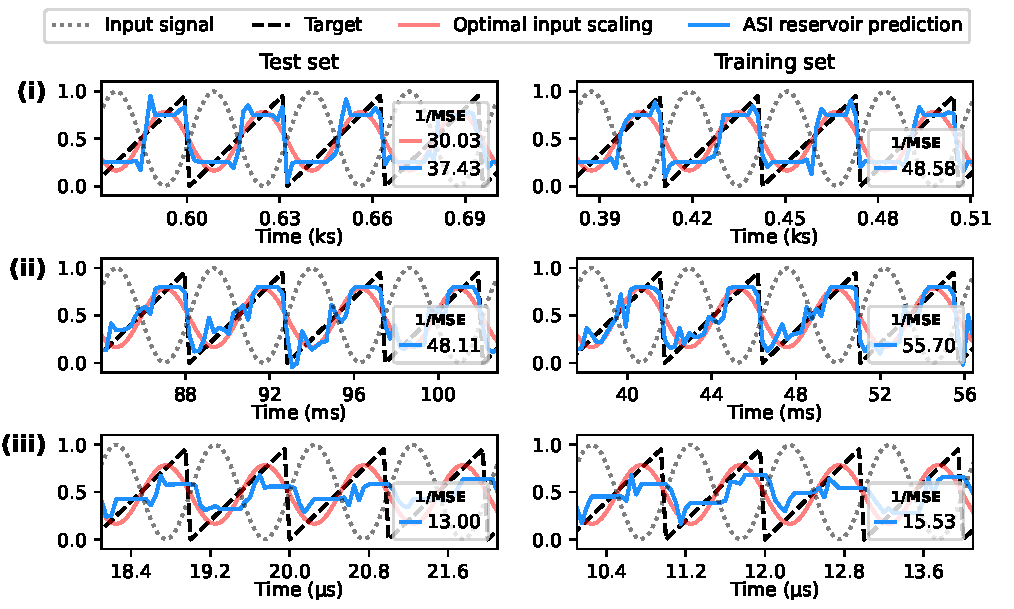
\includegraphics[width=\linewidth]{3_RC_OOP/Thermally active/Transformation/freq-magn/baseline/details.pdf}
	\vspace{-2.5em} % Looks more natural for this figure
}{
	\label{fig:3:Transformation_freq-magn_baseline}
	Monte Carlo simulations of a sine-to-sawtooth signal transformation performed by a thermally active $11 \times 11$ OOP square-lattice ASI reservoir.
	The top panel shows the inverse mean squared error $1/\MSE$ as a function of the input magnetic field frequency $f$ and amplitude $B_1$, with constant $B_0 = \SI{-0.35}{\milli\tesla}$, averaged over 5 runs with random $\sigma(\EEA)=\SI{5}{\percent}$ defects.
	Higher (lower) values in yellow (purple) indicate better (worse) performance.
	The black contours correspond to $1/\MSE \sim 30$, encompassing regions where the reservoir performs better than the linear transformation of the original input signal.
	In the top panel, several points are indicated with Roman numerals, corresponding to the bottom panels which show a temporal view of the transformation.
	There, the input sine-wave signal (grey dotted curve) and target sawtooth signal (black dashed line) are shown, alongside the prediction with and without the reservoir (blue and red curve, respectively).
}
\vspace{-1em}

To better capture the slope of the sawtooth, a higher input frequency is required.
It turns out that a rather broad range of well-performing input frequencies exists between $f \approx \SIrange{10}{e3}{\hertz}$, in combination with a maximum field magnitude $B_1 \approx \SI{0.2}{\milli\tesla}$, as indicated by the symbol \textsf{(ii)}.
Such a broad range of usable frequencies was to be expected considering the logarithmic nature of the relaxation dynamics.
At these frequencies, the waveform more closely resembles a sawtooth.
Still, the waveform is quite noisy due to the stochastic nature of the reservoir dynamics.
While the bottom of the sawtooth is captured rather well, the top exhibits a plateau which coincides with the minimum of the input sine wave, meaning the system is still given slightly too much time to relax. \par
Increasing the frequency further has a negative impact on the transformation, as is the case for \textsf{(iii)}.
The system becomes increasingly unable to approach the $\mavg \approx 0$ state and can only respond to the input when it is sufficiently strong, as evidenced by the sloped $1/\MSE=30$ border that separates points \textsf{(ii)} and \textsf{(iii)} in the top panels of~\cref{fig:3:Transformation_freq-magn_baseline}.
Instead, while there is still some periodic structure visible in the waveform generated by reservoir \textsf{(iii)}, it is dominated by noise since only a few random magnets will switch in the limited available timeframe.

\paragraph{Field magnitude range}
The minimal field magnitude $B_0$ for this system without gradient was set to \SI{-0.35}{\milli\tesla}.
This was determined through a similar parameter sweep as in~\cref{fig:3:Transformation_freq-magn_baseline}, but sweeping over $B_0$ and $B_1$ instead.
A constant frequency $f=\SI{100}{\hertz}$ was chosen, corresponding to the timescale at which this system reaches $\mavg \approx 0$ (\cref{fig:3:OOP_relaxation}, panel 8).
The results of this parameter sweep are presented in~\cref{fig:3:Transformation_magn-magnmin}, from which the optimal performance $B_0=\SI{-0.35}{\milli\tesla}$ was deduced.

\vspace{-1em}
\sidefig[0.53]{3_RC_OOP/Thermally active/Transformation/magn-magnmin/averaged.pdf}{
	\label{fig:3:Transformation_magn-magnmin}
	Inverse mean squared error $1/\MSE$ of a sine-to-sawtooth signal transformation using a thermally active $11 \times 11$ OOP square-lattice ASI, as a function of the input magnetic field range $B_0 \rightarrow B_1$ at a constant input frequency $f=\SI{100}{\hertz}$.
	Averaged results are shown over 5 runs with random $\sigma(\EEA)=\SI{5}{\percent}$ defects.
	Higher (lower) values in yellow (purple) indicate better (worse) performance.
	The black contours correspond to $1/\MSE \sim 30$, encompassing regions where the reservoir performs better than the linear transformation of the original input signal.
}

A point symmetry is visible about the origin of~\cref{fig:3:Transformation_magn-magnmin}: $\MSE(B_0, B_1) = \MSE(-B_0, -B_1)$.
The reason for this is the planar symmetry of the ASI, whose operation remains identical when it is flipped upside down.
While the optimal input frequency often remains of a similar order of magnitude regardless of the transformation --- since the frequency is mostly dictated by the relaxation dynamics --- the optimal range of input field magnitudes is highly dependent on the desired transformation.
For example, performance is somewhat reduced along the $B_0 = -B_1$ diagonal for the sine-to-sawtooth transformation considered here because this choice of input puts the sharp drop of the sawtooth at the moment when the input field is zero.
Other transformations can behave very differently: this kind of $\MSE(B_0, B_1)$-map can be used to identify their optimal input field range at a given frequency.

\paragraph{Gradient}
The previous discussion on input frequencies and magnitudes used a system without a \xref{property gradient}.
By making the magnets on one side of the system bigger than on the other side, the relaxation timescales can be spread out throughout the system, introducing more variation between the single-column readout nodes.
Quantitatively, a gradient $\Gamma$ means that the net OOP anisotropy $\EEA$ and magnetic moment $\mu$ on the right (left) side of the lattice are a factor $\Gamma$ higher (lower) than their average value throughout the ASI.
The varying magnetic moment $\mu$ also affects the NN MS coupling: the previously stated constant value of $\EMC = 2.5 \kBT$ now corresponds to the MS coupling between NN if their moment $\mu$ would be equal to the average magnetic moment $\llangle \mu \rrangle$ throughout the ASI.

\vspace{-1em}
\sidefigs[0.53]{3_RC_OOP/Thermally active/Transformation/grad-magn/freq1/averaged.pdf}{3_RC_OOP/Thermally active/Transformation/grad-magn/freq1/details.pdf}{
	\label{fig:3:Transformation_grad-magn_freq1}
	Impact of the \xref{property gradient} $\Gamma$ on the performance of a \SI{1}{\hertz} sine-to-sawtooth signal transformation by an $11 \times 11$ OOP square-lattice ASI reservoir.
	The top panel shows the inverse mean squared error $1/\MSE$ as a function of the gradient $\Gamma$ and amplitude $B_1$, with constant $B_0 = \SI{0}{\milli\tesla}$, averaged over 5 runs with random $\sigma(\EEA)=\SI{5}{\percent}$ defects.
	Higher (lower) values in yellow (purple) indicate better (worse) performance.
	The black contours correspond to $1/\MSE \sim 30$, encompassing regions where the reservoir performs better than the linear transformation of the original input signal.
	The panel at the bottom provides a temporal view of the transformation for a gradient $\Gamma = \SI{52}{\percent}$ and $B_1=\SI{0.45}{\milli\tesla}$, showing the input sine-wave signal (black dotted curve) and target sawtooth signal (black dashed line) alongside the prediction with and without the reservoir (blue and red curve, respectively).
}
\vspace{-0.5em}

The impact of the gradient is illustrated in~\cref{fig:3:Transformation_grad-magn_freq1} as a function of the input magnitude $B_1$\footnote{
	$B_0 = \SI{0}{\milli\tesla}$ was chosen to show it can be deduced from the figure by a very low $1/\MSE$ at $B_1 = B_0$.
}.
A low input frequency of $f=\SI{1}{\hertz}$ is used to assess whether the introduction of a gradient can improve upon the square-wave output that was generated at low frequencies in~\cref{fig:3:Transformation_freq-magn_baseline}.
Indeed, with the optimal gradient for this particular system, $\Gamma \approx \SI{50}{\percent}$, the transformation no longer resembles a square wave despite the low frequency.
For even stronger gradients, the performance drops again, as the range of anisotropies $\EEA$ in the system becomes too wide for an input signal to effectively induce dynamics throughout the whole system.
It can also be noted that the range of suitable input magnitudes $B_1$ expands as the gradient becomes more severe.
The reason for this is that the range of coercive fields of individual magnets in the system gets wider due to the property gradient.

\paragraph{System size and readout resolution}
Increasing the number of magnets $N$ in the ASI reduces the relative impact of thermal noise, since each readout node then averages over more magnets.
The central limit theorem states that the standard deviation of a mean scales as $1/\sqrt{N}$, so the value of $\mavg$ during relaxation will be more consistent in larger systems.
Hence, increasing the size of the system is expected to enhance the transformation quality as the final output then also becomes less noisy. \\\par
When each readout node represents the average magnetisation of one column, a square $N_x \times N_y$ ASI yields $p = N_x = N_y$ nodes ($\vc{x}(t) \in \mathbb{R}$).
However, as $p$ increases, the danger of overfitting increases as well~\cite{DeepRC_IonGating_Overfitting,lukovsevivcius2009reservoir}.
Overfitting is a general machine learning phenomenon that occurs when a model has too many trainable weights $\vc{w}$ for the limited data it has been given.
This causes the model to train on noise present in the data --- rather than on the general trend underlying that noisy data --- resulting in worse performance on the test set.
Since our thermally active OOP ASI reservoir is inherently noisy due to thermal fluctuations, overfitting is a possible concern.
Overfitting is one reason for why data is typically split into a training and test set, as the $\MSE$ on the training set may be too optimistic a measure for the reservoir performance. \\\par

The transformation performance with such single-column readouts is shown in~\crefSubFigRef{fig:3:Transformation_size-magn}{a}, as measured by $1/\MSE$ on both the training and test sets as a function of the number of readout nodes $p=N_x=N_y$.
At small $p$, performance is similar on both the training and test sets.
However, as $p$ increases, the training performance improves more rapidly than the test performance --- at $p=100$, for instance, $1/\MSE \approx 120$ on the training set, whereas it barely surpasses 75 on the test set.
This is a clear indication of overfitting. \par
Overfitting can be avoided by limiting the amount of readout nodes: in this system, for example, multiple columns can be averaged together.
The performance with a total of $p=11$ such readout nodes is presented in~\crefSubFigRef{fig:3:Transformation_size-magn}{b} as a function of system size $N_x = N_y$ and the input magnitude $B_1$.
Contrary to the single-column readout, the performance is now equal between the training and test sets, reaching a maximum of $1/\MSE \approx 60$ for $N_x=N_y=30$, beyond which enlarging the system no longer significantly affects the performance.

\vspace{-1em}
\makeshiftfig{
	\includegraphics[width=\linewidth]{3_RC_OOP/Thermally active/Transformation/size-magn/resx==size/averaged.pdf}\\
	%\vspace{-1em}
	\includegraphics[width=\linewidth]{3_RC_OOP/Thermally active/Transformation/size-magn/resx=11/averaged.pdf}
	\vspace{-2.5em} % Looks more natural for this figure
}{
	\label{fig:3:Transformation_size-magn}
	Impact of system size on a sine-to-sawtooth signal transformation by an OOP ASI reservoir as measured by the inverse mean squared error $1/\MSE$ as a function of the input magnetic field magnitude $B_1$, averaged over 5 runs with random $\sigma(\EEA)=\SI{5}{\percent}$ defects.
	The input frequency and minimal magnitude were kept constant at $f=\SI{800}{\hertz}$ and $B_0=\SI{0}{\milli\tesla}$, respectively.
	Higher (lower) values in yellow (purple) indicate better (worse) performance.
	The black contours correspond to $1/\MSE \sim 30$, encompassing regions where the reservoir performs better than the linear transformation of the original input signal.
	In panel \textbf{(a)}, each column of the ASI constitutes an individual readout node, while in panel \textbf{(b)} the number of readout nodes was kept constant at 11 by averaging multiple columns together.
	The left (right) panels show performance on the test (training) set, to identify overfitting.
}
\vspace{-1em}

\paragraph{Double-frequency transformation}
% TODO: address JLeliaert's comment about task agnostic metrics
With an ASI that can perform a decent sine-to-sawtooth transformation, other transformations can be targeted without changing the ASI --- provided the input is applied with an appropriate strength and frequency.
Only the weights $\vc{w}$ of the readout layer have to be adjusted to reflect this new target.
For example,~\cref{fig:3:Transformation_freq-magn_SINESQ} shows results for a double-frequency sine wave as target function.
For this transformation, the best fit attainable with a linear scaling of the input signal --- the red line in the bottom panel of~\cref{fig:3:Transformation_freq-magn_SINESQ} --- is simply a constant.

\sidefigs[0.53]{3_RC_OOP/Thermally active/Transformation/freq-magn/target_SINESQ/Sweep20231023131601.pdf}{3_RC_OOP/Thermally active/Transformation/freq-magn/target_SINESQ/details.pdf}{
	\label{fig:3:Transformation_freq-magn_SINESQ}
	Transformation of a sine wave input signal into a double-period sine wave by an $11 \times 11$ OOP square-lattice ASI reservoir.
	The top panel shows the inverse mean squared error $1/\MSE$ as a function of the input frequency and amplitude $B_1$, with constant $B_0 = \SI{0}{\milli\tesla}$.
	Higher (lower) values in yellow (purple) indicate better (worse) performance.
	The black contours correspond to $1/\MSE \sim 8$, encompassing regions where the reservoir performs better than the linear transformation of the original input signal.
	The panel at the bottom provides a temporal view of the transformation for $f=\SI{0.5}{\hertz}$ and $B_1=\SI{0.25}{\milli\tesla}$, showing the input sine-wave signal (black dotted curve) and target double-frequency sine (black dashed line) alongside the prediction with and without the reservoir (blue and red curve, respectively).
}

For this ASI reservoir to accurately produce a double-frequency sine, the input frequency must not exceed a threshold frequency $f_\mathrm{c} \approx \SI{10}{\hertz}$.
The quality of the double-period sine quickly deteriorates above $f_c$, as the system dynamics can no longer keep up to accurately produce a sine of double that frequency.
It is no coincidence that this value is similar to the timescale at which $\mavg \approx 0$ in panel 8 of~\cref{fig:3:OOP_relaxation}, which shows the relaxation in the absence of external stimuli for this system.
The same cut-off at $f_c$ is observed (though not shown in a figure) when the target function is a square wave.

\subsection{Signal prediction task: chaotic Mackey-Glass oscillator} \label{sec:3:Thermal_Prediction}
A special kind of ``transformation'' is a signal prediction, where the target function $y(t) = s(t + \Delta t)$ is a transformation of the input signal offset through time.
Such a prediction task benefits from the fading memory property of a reservoir to better infer the future evolution of the signal, while it relies less on a reservoir's non-linearity~\cite{TaskAdaptivePRC,NeuromorphicFewShot}.
The particular signal we will be attempting to predict with the thermally active OOP ASI is the chaotic Mackey-Glass oscillator $\mathrm{MG}(t)$~\cite{MackeyGlass}, as this is a popular benchmark in literature~\cite{RotatingNeuronsRC,AdaptiveProgrammableRC,TaskAdaptivePRC,Moon_2021,JaegerHaasWireless,ArchitecturalMarkovianESN}.
It can not be written in closed form; instead, it is implicitly defined by the delay-differential equation
\begin{equation}
	\label{eq:3:MG}
	\frac{d\mathrm{MG}(t)}{dt} = \frac{\beta \mathrm{MG}(t - \tau)}{1 + \mathrm{MG}(t - \tau)^n} - \gamma \mathrm{MG}(t) \mathrm{,}
\end{equation}
which was discretised by a time step $\tau/1000$ using the integration of~\ccite[Appendix A]{MeasuringStrangenessAttractors}.
Typical values for the parameters $\beta=0.2, \gamma=0.1$ and $n=10$ were used.
For $\tau \gtrsim 16.8$, this system is chaotic~\cite{jaeger2001echo}: $\tau=23$ was used here to get sufficiently chaotic behaviour, though $\tau=17$ is a more common choice.
To extinguish transients after releasing the oscillator from its initial state $\big(\mathrm{MG}(t \leq 0) = 0.5\big)$, a first timeframe $t \leq 25\tau$ is discarded.
Meanwhile, the extrema attained during this initial timeframe were recorded, to allow a scaling of subsequent input to the appropriate field range between $B_0$ and $B_1$. \par
While the Mackey-Glass oscillator is not strictly periodic, its delay parameter $\tau$ still provides a characteristic timeframe for its oscillations.
Therefore, the specific transformation attempted here is written as
\begin{equation}
	s(t) = \mathrm{MG}(ft\tau) \mapsto y(t) = \mathrm{MG}((ft + h)\tau) \mathrm{,}
\end{equation}
where $f$ fulfils the role of a ``frequency'' to synchronise the Mackey-Glass oscillator with the reservoir's relaxation dynamics despite the non-periodic nature of the signal.
This also provides the definition of the ``offset'' $h$, a dimensionless measure for how far ahead the reservoir must predict. \\\par

The previous discussion regarding the signal transformation task demonstrated that many system parameters affect the transformation quality --- including the input frequency $f$, the input magnitudes $B_0$ and $B_1$, the size $N_x \times N_y$ of the ASI, the \xref{property gradient} $\Gamma$, the number of readout nodes $p$ \dots\,
Since the absolute values of $f$, $B_0$ and $B_1$ provide limited additional insight and are unrelated to the ASI itself, we will henceforth use Bayesian optimisation~\cite{BayesOpt_Mockus1975} over the $f \times B_0 \times B_1$-space to identify the optimal input characteristics for a given set of ASI parameters. \par % This was not done for the figures relating to the signal transformation task, as it would be prohibitively expensive to compute the optimal system parameters for each pixel in those figures.
This allows us to concentrate on the most critical variable for a prediction task: the offset $h$, whose impact is illustrated in~\crefSubFigRef{fig:3:Prediction_MG}{a} for three particular systems with a different size and \xref{property gradient}.
For the systems with a gradient, $\Gamma$ was also optimised during the Bayesian optimisation procedure, which typically yields $\Gamma \approx \SIrange{25}{30}{\percent}$, though less severe gradients also perform decently. \par
Most strikingly, the optimum MSE\footnote{
	\crefSubFigRef{fig:3:Prediction_MG}{a} uses $\MSE$ rather than $1/\MSE$, as $1/\MSE$ for $h=0$ is much larger than for other $h > 0$.
	Furthermore, it is most common in literature to use $\MSE$ when reported as a function of the offset $h$.
} exhibits both a minimum and a maximum as a function of the offset $h$.
The resulting wave-like appearance of $\MSE(h)$ --- typical for this kind of input signal~\cite{AdaptiveProgrammableRC,ForecastingNeuralODE} --- originates from the definition of $\mathrm{MG}(t)$ as a delay-differential equation~\eqref{eq:3:MG}.
The characteristic delay $\tau$ makes it easier to predict $\mathrm{MG}(t + \tau)$ --- a delay $\tau$ corresponds to $h=1$, which closely aligns with the observed minimum of $\MSE(h)$.
For larger offsets $h$, more such minima will appear near $h \in \mathbb{N}$, though they quickly become less pronounced since the oscillator is not strictly periodic over $\tau$.
The performance at $h=0$ presents the limit of what the thermally active ASI reservoir can achieve, due to the stochastic nature of the relaxation process it employs.
Unsurprisingly, this limit improves by adding a gradient and increasing the system size.

\vspace{-1em}
\xfig{3_RC_OOP/Thermally active/Prediction/MG.pdf}{
	\label{fig:3:Prediction_MG}
	Performance of a thermally active OOP square-lattice ASI on a prediction task for the Mackey-Glass oscillator, for ASI of different size and gradient $\Gamma$.
	The number of readout nodes is fixed at $p=11$ for the $11 \times 11$ systems and $p=10$ for the $20 \times 20$ ASI.
	\textbf{(a)} Mean squared error as a function of the offset $h$, for the reservoir prediction (blue) and a linear transformation of the original input signal (red).
	The ultimate performance limit of each reservoir, $\MSE(h=0)$, is indicated by the horizontal grey dotted line.
	\textbf{(b)} Comparison of waveforms generated by an $11 \times 11$ ASI without a gradient (left) and a $20 \times 20$ ASI with a gradient $\Gamma = \SI{10}{\percent}$ (right), both for an offset $h=1.4$.
}
\vspace{-0.5em}

The $11 \times 11$ ASI reservoir without gradient (blue) only outperforms a linear scaling of the input (red) for $h > 0.4$.
Including a gradient and enlarging the system improves the $\MSE$, though the gradient appears more impactful than the subsequent enlargement.
More importantly than just the $\MSE$, the resulting waveform is also of better quality, as~\crefSubFigRef{fig:3:Prediction_MG}{b} shows for $h=1.4$.
The smaller ASI without gradient struggles to reproduce the peaks of the desired waveform, as its magnets only respond to a narrow field range.
On the other hand, the larger ASI with an appreciable gradient $\Gamma \approx \SI{25}{\percent}$ contains magnets with various coercive fields, enabling it to capture both the peaks and valleys, since these are likely to respectively coincide with low and high input fields.
%Besides the peaks and valleys, also the relatively constant $y(t)$ from $t=\SIrange{0.732}{0.736}{\second}$ is captured decently by the reservoir.

\subsection{Comparison with other reservoirs}
Generally speaking, our thermally active OOP ASI achieves an $\MSE$ of roughly 0.015 on both the sine-to-sawtooth transformation and the Mackey-Glass prediction task.
This performance is on par with several other magnetic reservoirs.
For instance, with a network of magnetic nanorings, an MSE of $\approx 0.014$ has been reported for the same transformation~\cite{Vidamour2023}.
Comparable results have been obtained with an artificial spin-vortex ice, which achieves $\MSE \approx 0.019$ for a sine-to-sawtooth transformation and $\MSE \approx 0.01$ for a Mackey-Glass prediction at an offset $k \approx 1.4$~\cite{gartside2022reconfigurable}.
Furthermore, combining multiple in-plane square and pinwheel ASI reservoirs in series has yielded $\MSE \approx 0.011$ for Mackey-Glass with $k \approx 0.8$ and $\MSE \approx 0.01$ on a sine-to-sawtooth transformation~\cite{AdaptiveProgrammableRC}. \par
Reconfigurable reservoirs can achieve better results as they are able to adapt to the task at hand.
One example of these is a skyrmion/conical reservoir~\cite{TaskAdaptivePRC}, which obtains a better sine-to-sawtooth transformation ($\MSE \approx \SIrange{e-4}{3e-7}{}$) and Mackey-Glass signal prediction ($\MSE \approx 0.0037$), though only at very low temperature $T = \SI{4}{\kelvin}$.
Above room temperature, $\MSE \approx 0.018$ was reported for an offset $k \approx 0.25$, closely matching the performance of our ASI reservoir. \par
Various non-magnetic physical reservoirs have also been benchmarked using these same tasks.
A carbon nanotube reservoir, for example, has been used to get $\MSE \approx 0.008$ on a sine-to-sawtooth transformation~\cite{CarbonNanotubeRC}.
Nanowire networks~\cite{NanoarchitectonicAtomicSwitch,RC_NNN} appear to achieve similar performance, as does the use of molecular vibration dynamics for reservoir computing~\cite{FewMoleculeReservoir}.
Chemical dynamics can also be utilised as a reservoir; for example, the use of electrochemical currents in a solution has yielded an $\MSE$ of $\approx 0.002$ for the sawtooth transformation task~\cite{ElectrochemicalPRC}. % 0.002 for polyoxometalate. For water, $\MSE \approx 0.04$.
Abstract echo state networks do outperform our system, as they have reportedly achieved $\MSE \approx 0.006$ for a very far future prediction of $k \approx 5$~\cite{Moon_2021}. % They gets NRMSE of 0.045 for their single-reservoir ESN, which corresponds to MSE 0.002, but their definition divides the normal MSE by the average square deviation, which is never more than 0.25. So the correspondence is quite vague.

\subsection{Summary}
By harnessing the spontaneous relaxation dynamics of thermally active OOP ASI, this type of system can be used as a reservoir thanks to its gradual response to external stimuli.
While this working principle inevitably suffers from thermal noise, which imposes a limit to the achievable performance, the extent of this noise can be greatly reduced by enlarging the system.
The computational capability of this system can be further boosted by including a property gradient.
Ultimately, the performance of thermally active OOP ASI is comparable to many other single reservoirs, on both signal transformation and prediction tasks.
A major advantage of thermally active ASI is that it can respond to a wide range of input frequencies --- spanning two orders of magnitude or more --- owing to the logarithmic nature of its relaxation dynamics.
Still, manufacturing thermally active ASI remains challenging, as this requires great control over the effective OOP anisotropy, which must not exceed several tens of $\kBT$.

% MSE is not an ideal parameter, should use something that accounts more for the general shape, because plateaus can have equal weight as noise, while they are visually quite different.

\newpage
\section{Reservoir computing in non-volatile out-of-plane ASI}
We now turn our attention to non-volatile ASI, to show that an ASI need not be thermally active to use it for reservoir computing.
When the energy barrier $\EEA$ of a magnet is significantly higher than the thermal energy $\kBT$, the N\'eel-Arrhenius switching law implies that it will remain stable over any reasonable timescale in the absence of external perturbations.
For example, a magnet with $\EEA > 40 \kBT$ will most likely remain stable for multiple years.
Therefore, non-volatile ASI is easier to construct than thermally active ASI, as great control over the perpendicular anisotropy is not required --- the anisotropy just has to be sufficiently large.
Throughout this section, we will develop, examine and discuss a ``clocked'' input protocol for non-volatile ASI that exhibits promising memory capacity.

\paragraph{Magnetostatic interaction}
Note that a ``non-volatile'' system is not the same as a non-interacting system.
While a low magnetostatic coupling $\EMC \ll \EEA$ results in a frozen system, a sufficiently high coupling will still induce spontaneous ordering, albeit only locally as the high anisotropy renders domain walls immobile.
Recall in this regard the five regions previously outlined in~\cref{fig:3:OOP_relaxation_continuous}.
Because of the high anisotropy $\EEA$, the superparamagnetic region~$\mathrm{V}$ and perfectly ordered region~$\mathrm{IV}$ are not relevant.
Instead, non-volatile ASI only exhibit two regimes: one where the magnetostatic coupling is sufficiently strong to overcome the energy barrier $\EEA$, and another where it is not.
These respectively correspond to region~$\mathrm{III}$~and~$\mathrm{I}$, while region~$\mathrm{II}$ is simply a smooth transition between these two regimes.
If, however, the RC input method does not cause significant local deviations from the ground state --- by for instance using domain wall motion for computation --- then these two regimes are equivalent from an RC perspective. \par

% Nomenclature: thermally active ASI has low energy barriers that allow the domain walls to move by thermal fluctuations, as all interactions are on the order of several $\kBT$. Spontaneously relaxing ASI just has a sufficiently strong MS interaction for domains to form, but domain walls will remain fixed in place when $\EMC$ or $\EEA$ is high. \par
% Achieving computation in a frozen system (i.e., region~$\mathrm{I}$) requires careful tuning of the strength of the input stimulus and the $\EMC/\EEA$ balance.

While the thermally active ASI typically had a MS coupling $\EMC \lesssim 10\kBT$, as was determined from the MFM images in~\cref{fig:3:MFM_grid}, such low coupling will be insufficient in non-volatile ASI.
For deterministic switching, both the anisotropy $\EEA$ and magnetostatic coupling $\EMC$ must be sufficiently high, say $\gg 40 \kBT$.
Increasing the magnetostatic coupling beyond $10\kBT$ should not present a significant practical issue, as the inclusion of a separate ferromagnetic layer above the magnets can significantly increase the MS coupling by focusing the stray fields onto nearby magnets~\cite[Supp. 10]{KUR-24}.

\paragraph{Uniform external field}
While it was possible to achieve decent signal transformation in thermally active OOP ASI by using a uniform external field, this approach is no longer viable in non-volatile ASI.
They lack the intrinsic relaxation dynamics that RC in thermally active ASI relied on, so a fundamentally different input method will be required.
In a non-volatile system, the temporal dimension is irrelevant, as a magnet will either switch within a reasonable timeframe or it will not.
Therefore, we must instead make use of the spatial dimensions of an ASI to perform RC.
Rather than pulling the system away from equilibrium and expecting it to evolve back to the ground state all by itself, we can instead use the domain structure for computation.

\subsection{Two-step input protocol: clocking}
To achieve control over the domains, we can take inspiration from the ``clocking'' protocol proposed by Jensen~\etal~\cite{clocking-protocol}, which can move domain wall boundaries in IP pinwheel ASI in discrete steps~\cite{SnakesInThePlane}.
While our square-lattice OOP ASI is very different from the pinwheel lattice, both exhibit domains, though these are superferromagnetic in pinwheel ASI rather than antiferromagnetic.
As such, some key concepts can be carried over, but the specific realisation of input and readout will have to be altered significantly to make such a clocking protocol work well for OOP ASI. \par
To achieve clocking, Jensen~\etal~\cite{clocking-protocol} applied an external magnetic field in a well-chosen direction to selectively affect one of the two pinwheel sublattices at a time, and then changed the field direction to affect the other sublattice.
By carefully tuning the field magnitude, only the magnets at the boundary of a domain --- or at the edge of the ASI --- will switch.
This is possible because those magnets have a lower effective energy barrier $\EBeff$ than magnets in the bulk of a domain.
Such a two-step clocking protocol therefore allows domain wall boundaries to advance one step at a time, while avoiding saturated magnetic states that would result from a stronger input. \par
The key takeaway from this concept is that two key factors are necessary if one wants to achieve controlled domain wall movement in any ASI~\cite{MAES-24}.
\begin{itemize}
	\item The input method must lift the degeneracy between the ground states --- in pinwheel ASI, a global in-plane field readily distinguishes between the four types of superferromagnetic domains.
	\item At least two independently addressable sublattices should exist to prevent avalanches --- in pinwheel ASI, two sublattices exist whose magnets are perpendicular to each other, enabling selective manipulation via in-plane fields.
\end{itemize}
Let us now consider the specifics how this can be achieved in a square-lattice OOP system.
This system is quite different from the IP pinwheel lattice used by Jensen~\etal~\cite{clocking-protocol} and will therefore require a different input method than just applying uniform fields at well-chosen angles.

\paragraph{Distinguishing between the degenerate ground states}
\subparagraph{Uniform field}
A uniform external field, as was successfully used in thermally active ASI, does not fulfil the first requirement.
It can not distinguish between the two checkerboard ground states, as it affects domains of both types equally and can therefore not be used in a clocking protocol.
In fact, a uniform field is not suited for RC in any non-volatile ASI that does not exhibit superferromagnetic domains, as it simply causes the magnetisation of low-$\EBeff$ magnets to align with the external field.
Any subsequent input cycle of opposite sign would either be too weak to have any additional effect, or be strong enough for the previously switched magnets to switch back, after which the same unremarkable process can repeat.
Regardless, a uniform field will not obtain the much coveted fading memory, precluding its use for RC in this system.
Hence, for an input protocol to induce desirable dynamics in non-volatile ASI, it must be specifically tailored to the lattice geometry.

\subparagraph{AFM input}
In the specific case of square-lattice OOP ASI, the two degenerate domain types can be separately addressed by applying an AFM ``checkerboard'' field --- a spatially alternating up/down external field where each magnet experiences an oppositely oriented field compared to its nearest neighbours\footnote{
	A practical realisation of such an AFM stimulus could be based on SOT induced by diagonal current lines, such that successive diagonals carry oppositely oriented currents, resulting in the required checkerboard pattern.
	Care must be taken, however, that this input is compatible with the AHE readout, which requires a full conducting layer rather than individual diagonal current lines.
	Since we focus on the theoretical potential of OOP ASI for RC, any additional practical considerations are beyond the scope of this thesis.
	% See rudimentary figure 20250403 for global vs clocked AFM input concept.
	% For global AFM input, the concept is to use a "snake" diagonal current line to get the alternating +/- checkerboard ordering, but the AHE underlayer is problematic as it enables short-circuiting such that the current does not follow the snake.
	% For clocked AFM input, the concept is to use "diagonally interlaced fingers" and only run current through half of them to get the clocking. This should be mostly compatible with the AHE, though uneven current distribution may be a concern.
}.
This alternating field temporarily lifts the degeneracy between the two domain types while the input is applied, hence promoting domains of one type at the expense of the other.
Information can then be encoded into the system by mapping a positive input value to one domain type, while a negative input corresponds to the other.

\subparagraph{AFM readout}
The readout method must be able to pick up on the changes induced by the input for there to be a meaningful input-output relation to perform RC with.
In our case, using the domain types for computation requires a readout method that can distinguish between the ground states.
This precludes the usage of a local $\mavg$ readout, as used for the thermally active system, nor can the order parameters $\qNN$ be used.
Instead, the domain type of each magnet will henceforth be used as the readout quantity, by mapping the two equivalent domain types to the values $\pm 1$.
Recall that it is theoretically possible to determine the state of all magnets in a small ASI from AHE measurements~\cite[Supp. 7]{KUR-24}.
Hence, such an AFM readout is practically achievable since it only requires a multiplication of the state of each magnet by $\pm 1$, depending on their location in the ASI. \par
To turn these individual magnetic states into a robust output vector, we will once again use averaging to avoid overfitting.
Since the $x$- and $y$-axes are equivalent, this is done via ``squinting'' --- effectively dividing the ASI into a coarser square lattice and averaging the states of $k \times k$ magnets for each readout value.
Hence, absolute values $<1$ indicate the presence of a domain boundary and it is even possible to distinguish between straight domain walls, corners and other features based on these averaged readout values.
Since there are $\approx N/k^2$ readout values, overfitting can be avoided by choosing $k$ sufficiently large.
Typically, we use rather small ASI just like we did for thermally active ASI, so $k=2$ is often a good choice for systems up to $20 \times 20$ magnets.

\paragraph{Avalanches and saturation}
The previously discussed AFM input method, which applies a spatially alternating up/down field, is insufficient to achieve controlled domain wall movement.
Because it applies a global stimulus, it easily triggers avalanches of switching magnets, rather than stepwise domain wall motion.
This occurs because most domain wall magnets all experience a similar effective energy barrier $\EBeff$, regardless of their location.
Hence, when the input is strong enough to move a domain wall by one lattice unit, the local environment at this new location is unlikely to be sufficiently different to impede further motion.
As a result, within a single input cycle, domain walls continue moving until they either annihilate, reach the system's edge, or encounter an insurmountable defect. \par

% In this regard, the AFM input method is not fundamentally different from the uniform input strategy we previously dismissed. Both simply provide each magnet with a preferential orientation, with only high-anisotropy magnets refusing to switch. Given this similarity, one might be inclined to consider them mathematically equivalent when paired with their respective readout methods. However, while both methods ultimately lead to saturation and are therefore unsuitable for RC, they differ in how they affect the microstate of the system when the magnetostatic interaction is appreciable. \par Compared to the AFM input method, a uniform field must be far stronger to have any effect, as it has to switch all magnets to the highest-energy state where all magnets have the same magnetisation direction. While the AFM input method also just pulls magnets in a certain direction, it differs in that it pulls the ASI to one of the ground states. This allows it to achieve saturation already with a far weaker input, since it only needs to affect domain wall magnets which have just $\leq 3$ oppositely magnetized NN and are therefore stable with $\EBeff \propto \EEA + 2\EMC$, as compared to $\EEA + 4\EMC$ for bulk magnets. It is therefore far easier to propagate a domain wall through the system to switch the ASI to the opposite ground state, as compared to pulling the system away from this near-equilibrium state to a uniform state. \par Hence, the effect of both global input methods on the ASI is fundamentally different, even though they both achieve saturation near-instantaneously which precludes their usage for RC.
% Summary of the previous comment: Both the AFM input method and the uniform input impose a preferred magnetisation direction, leading to saturation and making them unsuitable for RC. However, they differ in how they interact with the system when magnetostatic interactions are significant. A uniform input requires a much stronger field to overcome the stability of bulk magnets, which have four anti-parallel NN. In contrast, the AFM input naturally drives the system toward one of its ground states and requires a weaker stimulus, as it primarily affects domain wall magnets which have fewer oppositely magnetised NN and are therefore easier to switch.

The fact that the AFM input can selectively influence domain walls is crucial, as it enables us to avoid saturation by introducing one last change to this input strategy.

\paragraph{Avoiding avalanches with a clocking protocol}
Saturation can be avoided by instead applying two sub-steps for each applied input value. As illustrated in~\cref{fig:3:Clocking_protocol}, the magnets are divided into two groups, akin to the black and white squares on a checkerboard.
In the first sub-step, the AFM stimulus is only applied to the first group, while the second sub-step only addresses the second group of magnets.
The strength and/or sign of the stimulus is determined by the input value.
We refer to this method as the \idx{two-step AFM clocking protocol}.
This way, since only half of the magnets are stimulated simultaneously, the other half is prevented from switching at the same time --- provided their anisotropy $\EEA$ is sufficiently high compared to the NN MS coupling $\EMC$.
The avalanches that plagued the global input strategies are thereby avoided. \par
For this to result in controlled domain wall motion, the strength of the input is of great importance.
If it is too weak, the magnets will not respond.
If the input is too strong, though, all magnets will follow the applied field and a global ground state will be reached within a single input cycle nonetheless.
However, a range of input strengths exists where only domain wall magnets respond to the input, since any domain wall magnet is less stable than a magnet in the bulk of a domain\footnote{
	Domain wall magnets, with 3 oppositely and 1 parallelly magnetised NN, experience $\EBeff = \EEA + \EMC$. Bulk domain magnets have 4 oppositely magnetised NN, and are therefore more stable with $\EBeff = \EEA + 2\EMC$.
}.
%This is no different from the global AFM input method, but that method had no way of stopping the domain wall movement after it had begun.
Hence, by combining an appropriate choice of input strength with the two-step protocol that prevents half of the magnets from switching, it is possible to move domain walls by only a few lattice sites at once. % by deterministically switching only domain wall magnets towards the applied field.

\xfig{3_RC_OOP/Nonvolatile/Clocking_protocol.pdf}{
	\label{fig:3:Clocking_protocol}
	 Illustration of the \xref{two-step AFM clocking protocol} for controlled domain wall movement in ASI.
	 The symbols $\bigodot$ and $\bigotimes$ respectively indicate that the external stimulus is such, that the magnet at that location would prefer an `up' or `down' magnetisation.
	 This example shows a $5 \times 5$ ASI, but the concept is analogous for other lattice sizes.
	 Each input cycle consists of two sub-steps that each affect a different set of magnets, arranged in a checkerboard pattern: only half of the magnets are stimulated at once.
	 Input cycle $A$ (associated with bit 0) and input cycle $B$ (bit 1) apply opposite stimuli.
}

To use this clocking protocol for RC, input values must be mapped to a certain magnitude of the input stimulus.
Since we intend to use of the stepwise growth (or shrinking) of domains over only one lattice unit at a time, it is most convenient to apply this two-step input protocol to binary input data.
Therefore, two cycles $A$ and $B$ are defined, associated with input bits `0' and `1', respectively. \par
Both cycles consist of two sub-steps, as illustrated in~\cref{fig:3:Clocking_protocol}.
Using the analogy of black and white squares on the checkerboard, the first sub-step of cycle $A$ causes magnets on black squares to prefer an `up' magnetisation, while the other magnets remain unaffected.
The stimulus is then removed, after which the second sub-step causes magnets on white squares to prefer a `down' magnetisation without affecting magnets on black squares.
These preferential magnetisation directions are illustrated in~\cref{fig:3:Clocking_protocol} by the symbols $\bigodot$ and $\bigotimes$.
Cycle $B$ is identical but promotes the opposite magnetisation direction for each magnet, in order to grow domains of the opposite type as compared to cycle $A$. \\\par
This clocking protocol, coupled with this definition of the input, readily provides basic memory in the system, as the previous few input bits become encoded in the size and location of the domains.
Since this clocking protocol relies on deterministic switching, the duration over which the sub-steps are applied is irrelevant\footnote{
	As time is irrelevant to non-volatile ASI, all simulations use a default duration of \qty{1}{\second} per input cycle.
}. \par
While this clocking protocol is likely not the only viable input method for non-volatile OOP ASI, we can at least say with certainty that simply applying a global uniform or AFM field would not yield any useful dynamics for RC.
In the remainder of this section, we will illustrate the behaviour of the clocking protocol and show that it yields desirable dynamics for RC.

\subsection{Illustrative examples}
To show that the \xref{two-step AFM clocking protocol} does indeed move domain walls step by step, independent of their orientation or precise location, we will now consider a few example systems.
This will illustrate that the growth of domains can be controlled as originally envisioned, while providing insight into the effect of system parameters on the domain wall motion.

\paragraph{Defect-free system}
First, for a clean illustration of the general behaviour of the clocking protocol, consider an example without any defects, i.e. $\sigma(\EEA) = \SI{0}{\percent}$.
The absence of defects results in a far more orderly domain wall motion than expected in a real system, where domain walls would be likely to remain pinned at high-anisotropy magnets.
The effect of subsequent clocking cycles on such a ``perfect'' system is shown in~\cref{fig:3:Clocking_clearly_EBstd0}.
The top half of this figure shows the magnetisation state of each magnet, while the bottom half shows the same states but instead visualises the two degenerate domain types as black and white.
% While diagonal domain walls stand out in the top panels as lines of the same colour, horizontal/vertical domain walls (e.g. in the centre of the ASI during the $B$ cycles) are harder to see.
Both are equivalent, but the domain representation is more insightful in this context since the entire appeal of this input method is controlled domain wall motion.
Therefore, only the domain representation will be shown in any subsequent figures.

\makeshiftfig{
	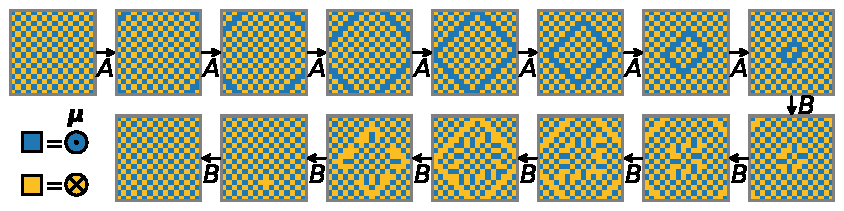
\includegraphics[width=\linewidth]{3_RC_OOP/Nonvolatile/Clocking_clearly_EBstd0_moments.pdf}
	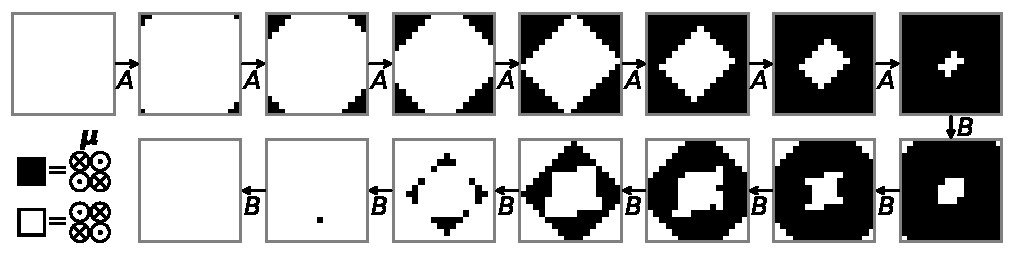
\includegraphics[width=\linewidth]{3_RC_OOP/Nonvolatile/Clocking_clearly_EBstd0_domains.pdf}
	\vspace{-1.5em} % Looks more natural for this figure
}{
	\label{fig:3:Clocking_clearly_EBstd0}
	Evolution of a $16 \times 16$ OOP square-lattice ASI when using the \xref{two-step AFM clocking protocol} (for seven cycles $A$ and seven opposite cycles $B$).
	The moment orientation (\textbf{top}) and domain type (\textbf{bottom}) of each magnet are shown after each cycle was applied.
	The finite size of magnets was accounted for with $D_\mathrm{NM} = \SI{170}{\nano\metre}$ and $S_\mathrm{ASI} = \SI{200}{\nano\metre}$.
	System parameters were chosen such that $\EMC = 40 \kBT$ and $\EEA = 200 \kBT$, with $\sigma(\EEA) = \SI{0}{\percent}$.
	All magnets are initially magnetised in one of the antiferromagnetic ground states (white).
	The magnetic field used in the clocking cycles has a magnitude $B_\mathrm{ext} = \qty{3.78}{\milli\tesla}$.
}

The figure clearly shows the stepwise growth of domains following the application of each individual clocking cycle.
While cycle $A$ promotes the domain type that is coloured black in the figure, cycle $B$ promotes the white-coloured domains.
These domains nucleate at the corners of the ASI, because those magnets only have two neighbours so their effective energy barrier $\EBeff$ is at least as low as that of a domain wall magnet.
During subsequent cycles, any existing domains of the type promoted by the applied cycle then grow at the expense of the opposite domain type. \par
A very important property of this input method is that cycle $A$ and $B$ are not each other's inverse, even though they only differ by the sign of their applied fields.
In the figure, this is reflected in the fact that the states visited by $B$-cycles were not previously visited by $A$-cycles.
Since some information from previous input cycles is often retained in this manner, this property provides the much coveted fading memory that is of great importance to RC. \par
Even though this system is non-volatile and defect-free, it can still exhibit some stochasticity.
One clear example of this is found in~\cref{fig:3:Clocking_clearly_EBstd0}: even though the three magnets at the bottom right switch during the first $A$-cycle, they do not switch during the first $B$-cycle.
The reason for this is the relatively low MS coupling $\EMC=40\kBT$, due to which the input strength must strike a delicate balance to avoid switching magnets that are not part of a domain wall.
These events can be suppressed by increasing the MS coupling, though a stronger input is then also required. \par % \\\par

Note also that, during the $B$-cycles in~\cref{fig:3:Clocking_clearly_EBstd0}, the central white-coloured domain does not re-grow with the same Petit-Beurre-shape\footnote{
	The ``Petit Beurre'' is a French biscuit decorated with serrated edges and four corners in the shape of ears, schematically resembling the central white-coloured domain that appears during the $A$-cycles of~\cref{fig:3:Clocking_clearly_EBstd0}.
} it previously had during the $A$-cycles.
Instead, it appears to preferably grow in such a way that it ends up with mostly horizontal and vertical edges, rather than diagonal ones.
This is part of the general phenomenon that, in the two-step AFM clocking protocol, domain growth preferentially occurs at the corners of a domain. \par
To more clearly illustrate this phenomenon,~\cref{fig:3:Clocking_massive_seeded} shows a far larger ASI which was initialised in one ground state, apart from one ``seed'' magnet at the centre which is of the opposite domain type as compared to all other magnets in the system.

\vspace{-1em}
\makeshiftfig{
	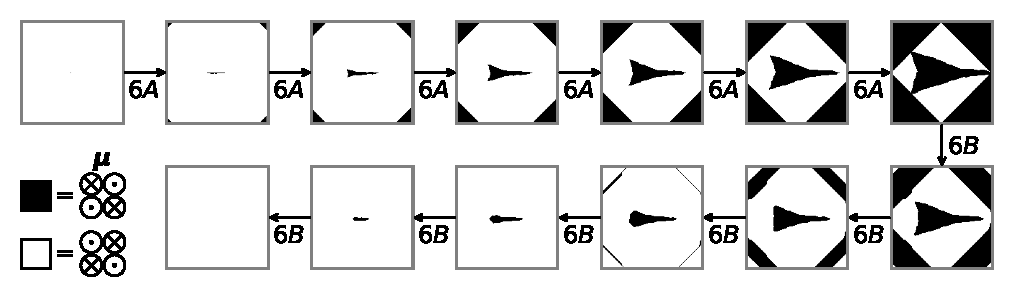
\includegraphics[width=\linewidth]{3_RC_OOP/Nonvolatile/Clocking_massive_seeded.pdf}
	\vspace{-1.5em} % Looks more natural for this figure
}{
	\label{fig:3:Clocking_massive_seeded}
	Evolution of a $141 \times 141$ OOP square-lattice ASI when using the \xref{two-step AFM clocking protocol} (for 36 cycles $A$ and 36 opposite cycles $B$).
	The domain type of each magnet is shown every six cycles.
	All magnets are initially magnetised in one of the antiferromagnetic ground states (white), apart from one magnet at the centre which started in the opposite state (black).
	The finite size of magnets was accounted for with $D_\mathrm{NM} = \SI{170}{\nano\metre}$ and $S_\mathrm{ASI} = \SI{200}{\nano\metre}$.
	System parameters were chosen to result in $\EMC = 40 \kBT$ and $\EEA = 200 \kBT$, with $\sigma(\EEA) = \SI{0}{\percent}$.
	The magnetic field used in the clocking cycles has a magnitude $B_\mathrm{ext} = \qty{3.78}{\milli\tesla}$.
}
\vspace{-1em}

During the first clocking cycle, one neighbour of the seed magnet will switch first, creating an asymmetry that causes the central domain to preferentially grow along that axis.
Magnets to the side of this elongated domain can also randomly switch, resulting in a gradual widening of the domain.
If this occurs at one of the domain's spearheads, whose tip is normally only 1 magnet thick, a small edge will be created that is 2 magnets long.
This is sufficient for the domain to fork into two diagonal directions since growth occurs preferentially at the corners of a domain.
This forking has occurred between the second and third panels of~\cref{fig:3:Clocking_massive_seeded}, but is a stochastic process: the right half of the domain in the figure did randomly fork. \par
Note also that, during the $B$-cycles in~\cref{fig:3:Clocking_massive_seeded}, white-coloured domains nucleate at the edges while the central white domain re-grows.
The white domains remain separated for about half as many $B$-cycles (18) as $A$-cycles were applied (36), at which time they reconnect and the rhombic black domain disappears.
Due to this imbalance, it is hard for domains to propagate far towards the centre when the input sequence contains equal amounts of each input bit.
Therefore, enhanced RC performance can be expected for systems with defects that allow domains to nucleate in the bulk of the system, or at least allow them to survive longer.

\paragraph{System with defects}
Any experimental realisation of OOP ASI will exhibit some degree of manufacturing defects, which are once again modelled by a normally distributed random anisotropy for each magnet in the ASI.
This results in more erratic states during successive steps of the clocking protocol as compared to the defect-free system from~\cref{fig:3:Clocking_clearly_EBstd0}.
However, contrary to the stochastic events mentioned before, the more erratic response caused by the disorder is reproducible and can therefore be used for computation. \par
The main reason for the more erratic response is that the difference between low- and high-barrier magnets in a system with defects can be substantial.
This often makes it impossible to find an input magnitude for which domain walls can propagate through any defect in the system without affecting magnets that are not part of domain walls.
Therefore, ``leaking'' can occur through low-barrier unstimulated magnets, which can spontaneously respond to the changing state of their neighbours even when they themselves are not stimulated~\cite{DisorderGroundStateASI}. % DisorderGroundStateASI says: "As expected, disorder allows dynamics to start inside the array at sites where ``loose'' spins with smaller switching fields are located."
This can be observed in~\cref{fig:3:Clocking_clearly_EBstd5} for an example with $\sigma(\EEA) = \SI{5}{\percent}$ and high MS coupling $\EMC = 200 \kBT$ compared to the anisotropy $\EEA = 100 \kBT$ to highlight leaking.

\makeshiftfig{
	%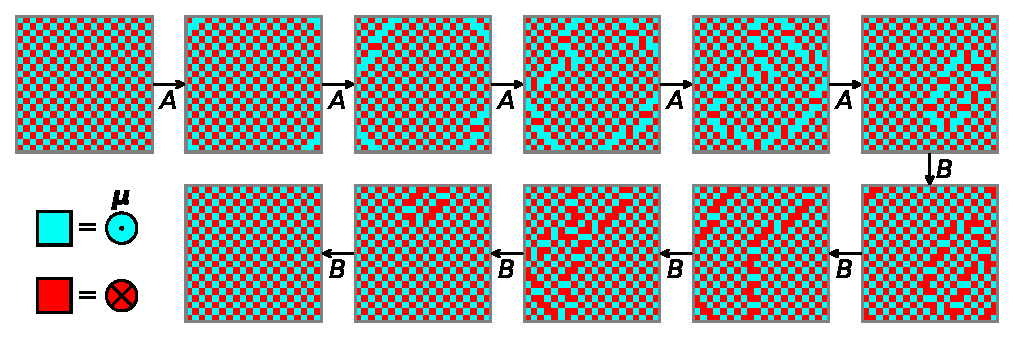
\includegraphics[width=\linewidth]{3_RC_OOP/Nonvolatile/Clocking_clearly_EBstd5_moments.pdf}
	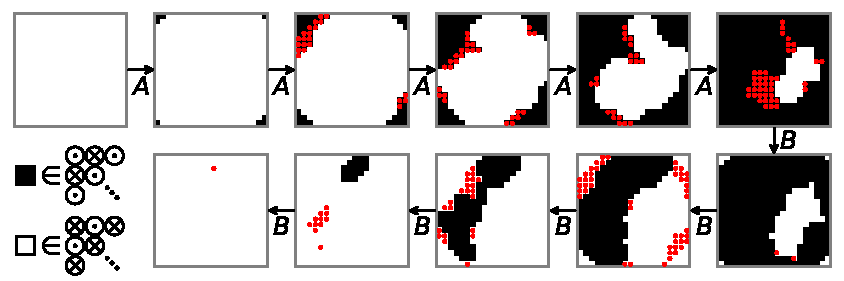
\includegraphics[width=\linewidth]{3_RC_OOP/Nonvolatile/Clocking_clearly_EBstd5_domains.pdf}
	\vspace{-1.5em} % Looks more natural for this figure
}{
	\label{fig:3:Clocking_clearly_EBstd5}
	Evolution of a $20 \times 20$ OOP square-lattice ASI when using the two-step AFM clocking protocol (for five cycles $A$ and five opposite cycles $B$).
	The domain type of each magnet is shown after each cycle.
	The finite size of magnets was accounted for with $D_\mathrm{NM} = \SI{170}{\nano\metre}$ and $S_\mathrm{ASI} = \SI{200}{\nano\metre}$.
	System parameters were chosen to result in $\EMC = 200 \kBT$ and $\EEA = 100 \kBT$, with $\sigma(\EEA) = \SI{5}{\percent}$.
	All magnets are initially magnetised in one of the antiferromagnetic ground states (white). The magnetic field used in the clocking cycles has a magnitude $B_\mathrm{ext} = \qty{5.5}{\milli\tesla}$.
}

Leaking can be mitigated by using a rather weak input, but this can make it impossible to switch some high-barrier magnets, rendering them frozen in their initial state.
This is to be avoided, as frozen magnets do not contribute to the fading memory of the system.
Alternatively, using a relatively strong input causes leaking but ensures that any magnet in the system can switch when required.
As long as domain walls do not move through too many unstimulated magnets per input step, leaking presents no issue.
It can even enhance RC performance, as it introduces asymmetry which is beneficial to the non-linearity of the system.
% Since leaking occurs due to low-barrier unstimulated magnets spontaneously switching in response to their neighbours, it is highly dependent on the magnetostatic interaction $\EMC$.

\paragraph{Energy balance}
As the ratio $\sigma(\EEA) \EEA / \EMC$ increases, so does the range of fields where low-anisotropy magnets can be switched in the bulk of a domain without significant leaking during stepwise domain wall propagation.
Such nucleation is beneficial for RC, in contrast to defect-free ASI where domain walls could only be injected at corners of the ASI.
%Fortunately from a fabrication perspective, systems with low $\EMC$ are typically easier to produce.
To illustrate the impact of $\EMC$,~\cref{fig:3:Clocking_clearly_EBstd5_EMC} compares a strongly-coupled system (a) with a weakly-coupled system (b). % a system with $\sigma(\EEA) \EEA / \EMC = 0.025$ (\crefSubFigRef{fig:3:Clocking_clearly_EBstd5_EMC}{a}) against one with $\sigma(\EEA) \EEA / \EMC = 0.25$ (\crefSubFigRef{fig:3:Clocking_clearly_EBstd5_EMC}{b}).
Indeed, nucleation occurs in the bulk of the weakly-coupled system because the disorder $\sigma(\EEA)\EEA=10\kBT$ is significant compared to $\EMC = 40 \kBT$, which also leads to far more irregular domain wall motion that encourages interactions between domain walls.

\vspace{-1em}
\makeshiftfig{
	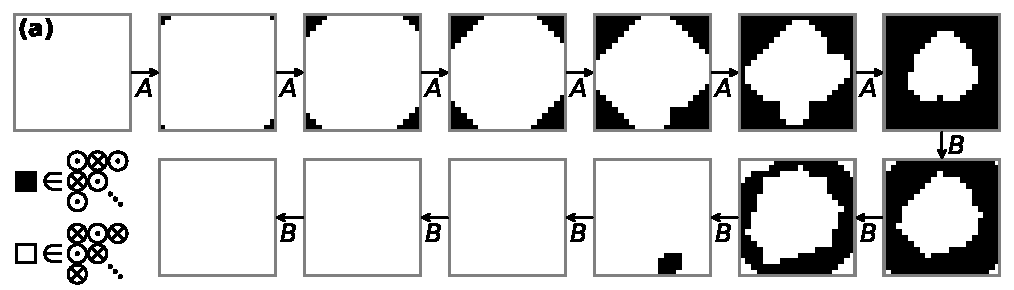
\includegraphics[width=\linewidth]{3_RC_OOP/Nonvolatile/Clocking_clearly_EBstd5_highEMC.pdf}\\
	\vspace{0.5em}
	\hrule
	\vspace{0.5em}
	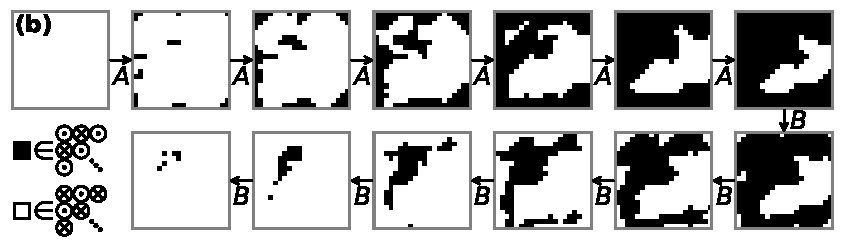
\includegraphics[width=\linewidth]{3_RC_OOP/Nonvolatile/Clocking_clearly_EBstd5_lowEMC.pdf}
	\vspace{-1.5em} % Looks more natural for this figure
}{
	\label{fig:3:Clocking_clearly_EBstd5_EMC}
	Evolution of the spatial distribution of domain types in a $20 \times 20$ OOP square-lattice ASI when using the two-step AFM clocking protocol (for six cycles $A$ and six opposite cycles $B$).
	All magnets are initially magnetised in one of the antiferromagnetic ground states (white).
	The finite size of magnets was accounted for with $D_\mathrm{NM} = \SI{170}{\nano\metre}$ and $S_\mathrm{ASI} = \SI{200}{\nano\metre}$.
	System parameters were chosen to result in $\EEA = 200 \kBT$, with $\sigma(\EEA) = \SI{5}{\percent}$.
	\textbf{(a)} System with high magnetostatic interaction $\EMC = 400 \kBT$, requiring an external input magnitude $B_\mathrm{ext} = \qty{11.2}{\milli\tesla}$ for controlled domain wall movement.
	\textbf{(b)} System with low MS interaction $\EMC = 40 \kBT$ and $B_\mathrm{ext} = \qty{3.78}{\milli\tesla}$.
}
\vspace{-1em}

Most importantly, note that the $B$-cycles do not remove the existing domains as quickly in the weakly-coupled system.
They even survive for as many $B$-cycles as there were $A$-cycles applied, which is great for RC as it improves the balance between both cycles.
Because of these benefits of weakly-coupled systems --- \crefSubFigRef{fig:3:Clocking_clearly_EBstd5_EMC}{b} exhibits exactly the kind of erratic, yet controlled behaviour we have been looking for --- we will henceforth focus on systems with a low $\EMC/\EEA$-ratio to obtain significant defect rates.

\subsection{Reservoir computing}
Due to the binary nature of the clocked input protocol --- as each cycle either grows or shrinks domains of a particular type --- it is most straightforward to supply binary input. % The limitation of binary input will be further explored in~\cref{sec:3:clocking_input_encoding}.
As this precludes the usage of certain tasks like signal transformation, we will instead evaluate the performance of this clocking protocol by determining more general RC metrics that do not rely on scalar input.
As introduced in~\cref{sec:1:RC_metrics}, these include metrics based on matrix ranks as well as the so-called task-agnostic metrics.
In the following, these will first be used to evaluate performance for a typical ASI that serves as our baseline, after which their effect on several system parameters can be assessed by adjusting this baseline ASI.

\subsubsection{Baseline system}
The ASI we consider here as our baseline system contains magnets with a very large perpendicular anisotropy\footnote{
	Note that the values for $\EEA$ and $\EMC$ used here are not expressed as multiples of $\kBT$ because the initial research on non-volatile ASI was conducted before the practice of scaling these parameters by $\kBT$ was adopted.
	For this reason, $\EEA$ is provided in \SI{}{\electronvolt} and the metrics are presented as a function of the lattice parameter $a$ rather than the magnetostatic coupling $\EMC$.
} $\EEA = \SI{110}{\electronvolt} \approx 4255\kBT (\pm \SI{5}{\percent})$ and the same magnetic moment as the thermally active ASI ($\mu = \SI{2.5e-16}{\ampere\metre\squared}$), which was based on magnets with a diameter $D_\mathrm{NM} = \SI{170}{\nano\metre}$.
As these parameters are kept constant, the MS coupling $\EMC$ only depends on the lattice parameter $a$.
To avoid an unintentionally interconnected ASI as previously encountered in~\cref{sec:3:MFM}, a lower limit $a > D_\mathrm{NM} + \SI{25}{\nano\metre} = \SI{195}{\nano\metre}$ is imposed. \par
The high anisotropy guarantees a weakly-coupled system with a high $\sigma(\EEA)\EEA / \EMC$-ratio, which we previously suggested to be the most promising regime for RC.
Given the constant values of the aforementioned system parameters, two variables remain: the input strength and the NN MS interaction energy $\EMC$.
To determine their optimal values, the RC metrics will be determined for a range of external field magnitudes $B$ and lattice spacings $a$. \par
Note that, while domain wall propagation can be expected near a field magnitude $B \approx (\EEA + \EMC)/\mu$, it is not guaranteed that optimal RC performance will occur exactly at this value.
The clocking dynamics are sensitive to the precise input strength, and the presence of disorder broadens the range where the input has a meaningful effect.
This makes it harder to predict which input strength $B$ will result in the best performance, which can also be different for each metric.
Therefore, while the optimal field magnitude is predictable to some extent, it is also varied to ensure hitting the ``sweet spot'' for all metrics.

\paragraph{Matrix rank-based metrics}
Three matrix rank-based metrics can be calculated (\cref{sec:1:RC_metrics_KQ}): the kernel-quality $K$, generalisation-capability $G$ and computing capacity $C=K-G$.
The latter provides a general indication of how suitable a particular system is for reservoir computing.
\cref{fig:3:Clocking_Sweeps_binary_KQ} shows these metrics for the baseline system over a range of lattice spacings $a$ and field magnitudes $B$.
Recall that the maximum value of $K$, $G$ and $C$ is the number of readout nodes; here, a $20 \times 20$ ASI with $10 \times 10$ readout nodes --- each representing the average domain type of a $2 \times 2$ magnet cluster --- yields a maximum value of 100 for all three metrics.

\xfig{3_RC_OOP/Nonvolatile/Sweeps/Sweep20230208082817.pdf}{
	\label{fig:3:Clocking_Sweeps_binary_KQ}
	Kernel-quality $K$, generalisation-capability $G$ and computing capacity $C$ of a $20 \times 20$ OOP square-lattice ASI with $\EEA = \SI{110}{\electronvolt} \pm \SI{5}{\percent}$.
	Beyond the displayed range of lattice constants $a$ and input field magnitudes $B$, the metrics decrease.
	The corresponding magnetostatic coupling $\EMC$ ranges from $146\kBT$ (at $a=\SI{220}{\nano\metre}$) to $88\kBT$ (at $a=\SI{260}{\nano\metre}$), as the magnetic moment of each magnet is $\mu = \SI{2.5e-16}{\ampere\metre\squared}$.
	As readout, the average domain type of each $2 \times 2$ set of magnets is used, totalling 100 readout values.
	Hence, the highest possible value of $K$, $G$ and $C$ is 100.
}

Some noise is visible in the figure due to the random distribution of $\EEA$; for each set of parameters, a new randomly sampled value of $\EEA$ was assigned to each magnet.
The local noise level therefore reflects how impactful a $\sigma(\EEA) = \SI{5}{\percent}$ disorder is on the clocking dynamics and, by extension, on RC performance.
For example, near the maximum of the metric map in~\cref{fig:3:Clocking_Sweeps_binary_KQ}, the computing capacity $C$ may vary between approximately 50 and 80.
This suggests that, unless such defects can be reproducibly incorporated into the system, performance can vary significantly between various manufactured ASI samples. \par
The generalisation-capability $G$ is very low for any combination of $a$ and $B$, apart from a few outliers where the randomly sampled defect distribution results in uncharacteristically high values of $G$.
Because $C=K-G$ provides an indication of RC performance, a low $G$ is advantageous: it indicates that recent inputs have a far greater impact on the current state of the system than older input cycles.
In this baseline system, this low generalisation-capability allows the computing capacity $C$ to reach values as high as 80 out of 100. \par
Additionally, though not shown in the figure, it is worth noting that accounting for the finite size of magnets has no noticeable impact on RC performance, apart from shifting the entire metric map by roughly $\Delta a = \SIrange{20}{30}{\nano\metre}$ toward larger lattice constants as compared to a point dipole model. % If we want to show this as figures, compare Sweep20250325131714 vs. Sweep20250325105313.

\paragraph{Task-agnostic metrics}
Although the matrix rank-based metrics provide insight into how the system responds to various input patterns, they are relatively expensive to compute --- requiring as many input sequences as there are readout nodes (here: 100), with each sequence comprising many (here: 100) input values.
In comparison, task-agnostic metrics such as non-linearity and memory capacity can be determined using only several hundred random input values, making them considerably more efficient to compute.
Furthermore, while matrix rank-based metrics can serve as useful initial indicators of whether a system can exhibit promising dynamics for RC, they do not guarantee that a system is actually suitable for RC.
Task-agnostic metrics are more straightforward to interpret and provide a more accurate indication of a system's suitability for RC.
For example, the input method with a uniform field --- which was previously dismissed for non-volatile ASI --- achieves a moderate $C \approx 40$, but yields very low values for all task-agnostic metrics like non-linearity and memory capacity. % Matrix rank-based metrics should rather be seen as indicators of which systems do NOT give decent RC performance.
Therefore, to complement the findings from the previous paragraph, task-agnostic metrics were also determined for the baseline system over the same parameter range, as shown\footnote{
	The stability metric is also among the task-agnostic metrics proposed in~\cite{RC_TaskAgnosticMetrics_v2}, but is not shown here as it is not relevant to non-volatile ASI which do not spontaneously reach a ground state in the absence of input.
} in~\cref{fig:3:Clocking_Sweeps_binary_TA}. \par
Note that the non-linearity metric will naturally be lower for binary input than for the scalar input it was designed for.
The reason for this is that binary input offers only two possible values, making it generally easier to fit a linear model to the input-output relationship.
Therefore, the parity check metric is also shown, as it was specifically designed for binary input. % See ppt 20230207

\xfig{3_RC_OOP/Nonvolatile/Sweeps/Clocking_binary_TA_averaged.pdf}{
	\label{fig:3:Clocking_Sweeps_binary_TA}
	Task-agnostic metrics for the same input, readout and system parameters as in~\cref{fig:3:Clocking_Sweeps_binary_KQ} ($20 \times 20$ OOP square-lattice ASI with $10 \times 10 = 100$ readout nodes, $\EEA = \SI{110}{\electronvolt} \pm \SI{5}{\percent}$, $\mu = \SI{2.5e-16}{\ampere\metre\squared}$), over the same range of lattice spacings $a$ and input magnitudes $B$.
	The non-linearity is bounded in the range $[0,1]$, while the memory capacity and parity check have no upper limit.
}

Systems with stronger MS interaction behave more non-linearly, though only in a narrow range of input field magnitude.
The trade-off between non-linearity and memory capacity, which has been extensively discussed~\cite{dambre2012information,MemoryNonlinearityReservoirs,RC_BeyondMemoryNonlinearity,RC_unification} and reported in various systems~\cite{DynamicEmergence_NanomagneticSystem,RC_TaskAgnosticMetrics_v2,TaskAdaptivePRC}, is striking in this system as well.
As envisioned, the clocking protocol indeed yields a relatively high memory capacity, obtaining values $>2$ over a wide range of the parameter space.
The parity check reveals that, on average, the parity of the previous 3 input cycles can be recalled over a wide range of the metric map.
That the parity check reaches higher values than the memory capacity was to be expected, as it is specifically tailored to binary input data whereas memory capacity is more generally applicable to scalar data, though the parity check also includes a notion of non-linearity.
These metrics provide more insight than the matrix rank-based metrics, as they can directly be related to the performance of the system for certain tasks --- some tasks mostly rely on fading memory while others mostly require non-linearity, and yet others prefer a mix of both. \par
While $<3$ bits of memory may sound low, it is comparable to the memory capacity and parity check of other magnetic reservoirs~\cite{AdaptiveProgrammableRC,hon2021numerical,tsunegi2019STOforcedsyncRC,Venkat_2024,Vidamour_2022}. % AdaptiveProgrammableRC is similar when using a normal square ASI, but width-modulated and pinwheel ASI perform better.
Higher performance can be achieved by using general RC architectures like the rotating neurons reservoir~\cite{RotatingNeuronsRC} or the single dynamical node paradigm~\cite{appeltant2011information}, as for example used in~\ccite{Venkat_2024,Vidamour2023}.
However, here we only consider the performance of the clocked ASI by itself, as these architectures can be applied to any reservoir.

\paragraph{Effect of initial state}
The initial state of the system can, in some cases, influence RC performance.
While the initial state has little to no impact when the input is sufficiently strong, as the initial state gets washed out after several clocking cycles, it can significantly affect the results at lower input magnitudes.
The reason for this is that different initial states require different minimal input field magnitudes --- it is easier to switch a magnet when the ASI is in a uniform state than when it is in the AFM ground state. % Compare Sweep_230220_1_binaryInput_randomInit.out/Sweep20230220132509 with Sweep_230119_2_binaryInput.out/Sweep20230119153543
This is further complicated by defects, which may impede domain wall motion.
For example, when starting from the AFM ground state, domain walls must be injected from the edges and propagate throughout the system, whereas an initially uniform state will enable initial switches (i.e., domain wall nucleation) to occur throughout the bulk of the system.
Therefore, a field range exists where an ASI in the uniform state will respond to the input, while it would not if it were in the AFM ground state.
This range is broader for more strongly-coupled and disordered systems. \par
This effect is an example of how metric maps can be affected by other factors than just system parameters.
Therefore, to ensure consistency between the RC metric maps presented in this section, all simulations start from the AFM ground state\footnote{
	While the high anisotropy $\EEA$ prevents the system from spontaneously reaching the ground state, it can be forced to the ground state by applying a single clocking cycle with a stronger stimulus than used during computation.
}.

\subsubsection{Influence of defects on RC metrics}
We previously mentioned that disorder is beneficial to the RC capability of the system, but provided no evidence for this.
Now, RC metrics can be used to verify this claim: the task-agnostic metrics for a system without defects ($\sigma(\EEA) = \SI{0}{\percent}$) are shown in~\cref{fig:3:Clocking_Sweeps_binary_TA_EBstd0}. \par
While the memory capacity and parity check are still definitively non-zero, they are at least $\approx \SI{40}{\percent}$ lower than for a system with $\sigma(\EEA) = \SI{5}{\percent}$ defects.
Furthermore, while a region with near-unity non-linearity now exists, the overlap between parameter combinations that yield decent non-linearity and those that yield decent memory capacity remains rather limited. \\\par

\xfig{3_RC_OOP/Nonvolatile/Sweeps/Sweep20230124100320.pdf}{
	\label{fig:3:Clocking_Sweeps_binary_TA_EBstd0}
	Task-agnostic metrics for a defect-free system ($\sigma(\EEA) = 0$) with otherwise the same input, readout and system parameters as in~\cref{fig:3:Clocking_Sweeps_binary_TA} ($20 \times 20$ OOP square-lattice ASI with $10 \times 10 = 100$ readout nodes, $\EEA = \SI{110}{\electronvolt}$, $\mu = \SI{2.5e-16}{\ampere\metre\squared}$), over the same range of lattice spacings $a$ and input magnitudes $B$.
	The non-linearity is bounded in the range $[0,1]$, while the memory capacity and parity check have no upper limit.
}

While this shows that defects improve the memory capacity of the system, it does not prove that a defect rate $\sigma(\EEA) = \SI{5}{\percent}$ would be optimal.
To assess this,~\cref{fig:3:Clocking_Sweeps_binary_TA_EBstd} shows task-agnostic metrics for a range of defect rates $\sigma(\EEA)$ and input field magnitudes $B$ while the lattice spacing was kept constant.

\xfig{3_RC_OOP/Nonvolatile/Sweeps/Sweep20250327111551.pdf}{
	\label{fig:3:Clocking_Sweeps_binary_TA_EBstd}
	Task-agnostic metrics as a function of disorder $\sigma(\EEA) = 0$ with otherwise the same input, readout and system parameters as in~\cref{fig:3:Clocking_Sweeps_binary_TA} ($20 \times 20$ OOP square-lattice ASI with $10 \times 10 = 100$ readout nodes, $\EEA = \SI{110}{\electronvolt}$, $\mu = \SI{2.5e-16}{\ampere\metre\squared}$), over the same range of input magnitudes $B$, with $a=\SI{230}{\nano\metre}$ kept constant.
	The non-linearity is bounded in the range $[0,1]$, while the memory capacity and parity check have no upper limit.
}

The non-linearity quickly drops as the disorder increases; only systems with rather low disorder ($< \SI{10}{\percent}$) display an appreciable non-linearity, and only do so over a limited field range.
The memory capacity and parity check, on the other hand, benefit greatly from disorder.
Note that the first column in~\cref{fig:3:Clocking_Sweeps_binary_TA_EBstd} (i.e., $\sigma(\EEA) = 0$, a defect-free system), displays a far lower memory capacity or parity check performance than any system with defects ($\sigma(\EEA) > 0$).
The severity of these defects has no substantial impact on these two metrics; they remain reasonably high ($\gtrsim 2.5$ and $\gtrsim 3$, respectively) even for extremely severe defects beyond $\sigma(\EEA)=\SI{30}{\percent}$. \par
The optimal field range always remains centred around the same value, but broadens as the disorder increases.
This is a consequence of the greater spread of effective energy barriers throughout the ASI due to the increased disorder, widening the range of field strengths at which any of the magnets can switch.

\subsubsection{Alternative input encoding}
\label{sec:3:clocking_input_encoding}
The clocking protocol naturally lends itself to binary input\footnote{
	Generally speaking, a clocking protocol lends itself to as many possible input values as there are degenerate ground states in the system.
	In OOP ASI, this results in binary input (2 values).
	One could similarly imagine a quaternary input (4 values) for Pinwheel ASI, which exhibits superferromagnetic domains with 4 possible average magnetisation angles, though this is mere conjecture as binary input was used by Jensen~\etal~\cite{clocking-protocol} when demonstrating clocking in pinwheel ASI.
}.
For many real-world RC tasks, however, scalar input is preferable.
Within the limits of the clocking protocol, we propose two concepts to address this, though neither are desirable. \par
The first concept is to use an analog-to-digital conversion that encodes scalar values as integers represented as little-endian bytes consisting of 8 bits.
This is the natural habitat of conventional computers, but is not a viable solution here since the memory capacity of the system is less than one bit.
The non-linearity, on the other hand, was found to remain mostly unaffected, aside from a slight increase due to the larger input space (256 values as compared to 2 for binary input).
However, all things considered, this byte-wise method is not a viable alternative to binary input. \par
The second concept is to use the input magnitude as a scalar input, similar to the thermally active ASI.
However, non-volatile ASI only exhibit a non-trivial response to the input in a narrow range of field magnitudes.
Furthermore, one must take care to regularly apply both positive and negative cycles to keep the domain wall dynamics going.
Both of these factors complicate the input encoding. \par
Ultimately, both of these scalar input concepts were dismissed as they did not provide a desirable effect.

\subsection{Summary}
Achieving reservoir computing in non-volatile OOP ASI posed several challenges.
A uniform global input could not be used for RC, as it does not distinguish between the degenerate ground states.
This was solved by devising an input with the same checkerboard pattern as the AFM ground state.
However, applying a global AFM input did not yield usable dynamics since uncontrolled domain wall motion saturates the system in one of its ground states, erasing prior information present in the system.
This led us to formulate two basic requirements for using a non-volatile ASI as a reservoir: the input must lift the degeneracy of the ground states such that it can affect domain boundaries, and at least two independently addressable sublattices should exist to prevent avalanches. \par
Hence, a clocking protocol was developed that does not stimulate all magnets simultaneously.
More specifically, the system was divided into two interleaved sublattices, allowing the controlled propagation of domain walls.
Nonetheless, in the absence of defects, the information stored by this clocking protocol was rather limited as a large portion of the response was reversible and highly symmetric.
The reproducible disorder provided by defects --- within a specific ASI sample --- breaks the symmetry and creates more irreversible dynamics in the bulk of the system, thereby enhancing its computational capability.
This was reflected by an increased memory capacity ($\approx 1.5 \rightarrow 2.5$ bits) and parity check performance ($\approx 1.5 \rightarrow 3$ bits), though the maximum non-linearity decreased. \par
A limitation of the clocking protocol is that it only allows binary input, but for real-world applications scalar inputs are often more relevant.
It is, however, non-trivial to devise a scalar input protocol for non-volatile ASI.
In this sense, the thermally active and non-volatile ASI complement each other --- supporting analog and binary input, respectively.

\section{Conclusion}
We have numerically demonstrated the reservoir computing capability of both thermally active and non-volatile OOP ASI, each of which required very different input methods.
The spontaneous logarithmic relaxation of thermally active ASI towards the ground state results in a gradual response to external stimuli over a broad frequency range, which allowed us to use them as a sort of leaky integrator.
However, non-volatile ASI requires a more intricate input method in order to avoid avalanches, which led us to develop a clocking protocol that results in stepwise domain wall motion. \par
Since thermally active systems can readily process analog input, we evaluated their RC performance on a signal transformation and prediction task.
The binary character of the clocking scheme restricts its available tasks, so there we opted to use task-agnostic metrics instead.
Both systems achieved a performance comparable to other single reservoirs on their respective tasks and metrics.
Introducing spatial variation --- in the form of a property gradient in thermally active ASI and random disorder in non-volatile ASI --- was found to provide a richer output for both systems.
On a similar note, enlarging the lattice of thermally active ASI aids to reduce thermal noise which otherwise limits the attainable performance. \par
In conclusion, these two types of OOP ASI complement each other in the sense that they respectively support analog and binary input, for which they both achieved satisfactory results at benchmark tasks and metrics.
